\chapter{Process model application}
\label{chp:processmodelapp}
\todo{write chapter introduction}

    \section{Example process}
        \begin{figure}
            \footnotesize
            \center
            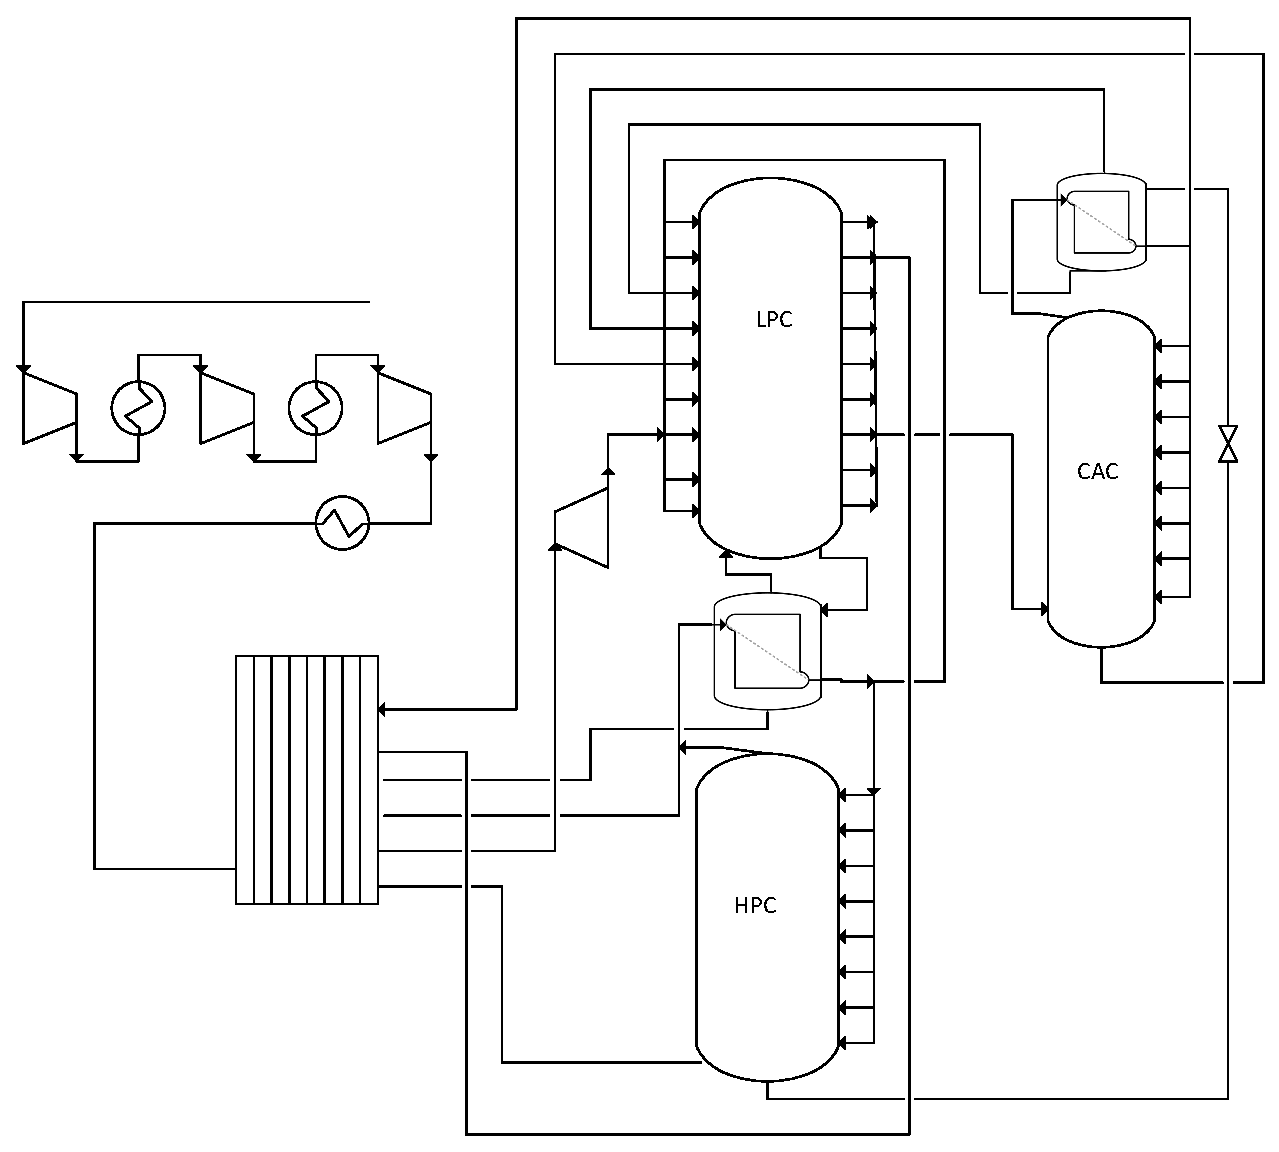
\includegraphics[width=\linewidth]{Pictures/ASU_superstructure}
            \caption{Example process superstructure.}
            \label{fig:opt:exppro}
        \end{figure}

        The developed models were combined to a process flowsheet for the cryogenic air separation process.
        As no specific process was being evaluated, the process configuration was modeled after an
        published example process flowsheet \cite{Kooijman.}. \Figref{fig:opt:exppro}
        shows the flowsheet considered henceforth. Air is drawn from the surrounding at ambient conditions
        and compressed with inter-cooling stages. Afterwards the entering process stream exchange heat
        with the product streams.

        The stream is then divided into two separate streams. One part is expanded in a turbine, and fed to
        the low pressure column (LPC) while the majority is fed to the high pressure column (HPC).
        Condenser and reboiler are combined in a single unit. A side column to the LPC generates pure
        argon. The condensate form the HPC is partially fed into the LPC. The oxygen rich sump product form the HPC
        is used to condensate the CAC top product, and afterwards fed into the LPC. From the reboiler side liquid oxygen
        is recovered from the process. From the top of LPC and HPC gaseous nitrogen is drawn. Liquid Argon is drawn from 
        the CAC condenser. 
        
        AS can be seen, this process is highly integrated with respect to energy and material streams. For both the
        steady-state and dynamic process model, the same separation sequence is considered. Compression and heat-exchange 
        are only explicitly modeled in the steady-state process. While the steady-state models do provide the possibility 
        to calculate pressure drops by means of an hydraulic model, they were assumed constant in all steady-state applications. 
        When using the dynamic models, hydraulic equations have to be considered. For the case of the ASU process different column 
        internals are often installed. The HPC as the smallest column can be economically operated as a trayed column, hence the 
        respective hydraulic and cost models were employed there. The LPC and CAC are mostly equipped with structured 
        packings. 
        
        Another difference in the steady-state and dynamic models was the considered superstructure. For optimizing the number 
        of separation stages, a maximum value needs to be guessed. In the steady-state case those were set to 40 for the HPC
        and 60 for the LPC and CAC respectively. With the steady-state results in mind, these were reduced to 25 for the HPC
        and 45 for LPC and CAC when constructing the dynamic process.  

    \section{Steady-state models}
            There are several ways in which a process model in general, and the steady-state models in particular can be used. 
    In this case, all models have been implemented with the use for operational and structural optimization 
    in mind. 
    
    This section begins, with a discussion of the degrees of freedom, coupled with feasible specifications. 
    Linked to this matter is the crucial question of model initialization, which is dealt with in the 
    subsequent section. Finally a look at different optimization setups concludes this section. 


    \subsection{Degrees of freedom}
        The equation systems presented above is comprised of $n_S n_C$ component balances and equilibrium
        equations, $2n_S$ summation equations and $n_S$ energy balances. This gives a total of $n_S (2n_C + 3)$
        equations. On the other hand there are $n_S$ temperatures and pressures, $2n_S$ molar flow rates,
        $n_S$ energy streams, and $n_S n_C$ vapour as well as and liquid concentrations. Additionally the feed flow rates
        compositions and temperatures and the side draw split fractions or flow rates appear as variables. The
        feeds and side draws would usually be specified, which leaves a total of $n_S (2n_C + 5)$ variables.

        The pressure profile of a distillation column is usually specified.
        In terms of unit operations this pressure drop is of high significance,
        as many columns can only be feasibly operated if the pressure drop does not exceed certain
        limits. In case of the ASU the production of Argon only became feasible as structured
        packings, which display a very low pressure drop, became available. This is due to the large
        number of theoretical stages required to attain the desired Argon purities.

        The energies $Q_i$ denote addition heaters or cooler on the respective stages. For all
        intermediate stages these values would be specified as well. If all energies are
        specified, that would -- along with the pressure profile -- sum up to $2 n_S$ specifications,
        which leaves $n_S (2n_C + 3)$ unknowns. As the number of equations and unknowns are the equal,
        this system is then well specified.

        In practice it is often challenging to correctly guess the condenser and reboiler heat loads in
        advance. This is especially true since they have a tremendous impact on the overall performance
        of the column. Hence it is often desirable to supply other specifications than the respective
        heat loads. To allow for such specification so called discrepancy functions can be introduced
        \cite{Henley.op.2011}, which replace the energy balance for the condenser and / or reboiler stage.

        One common specification is the so called reflux ratio $\nu^D = \frac{L_1}{V_1 + S_1^L}$ for
        the condenser, or the boil-up ratio $\nu^R = \frac{L_N}{V_N}$ for the reboiler.
        They are defined as the ratio of the molar flowrate sent back into the column over the
        product flowrate which leaves the column. For the reboiler this denotes a liquid stream,
        while for the condenser the product can be gaseous and liquid. Specifying this leads to
        \Eq{eq:reflux}{
            0 & = L_1 - \nu^D \cdot (V_1 + S_1^L), \\
            0 & = V_N - \nu^R \cdot L_N,
        }
        \ncg{\nu^R}{boliup ratio}{-}
        \ncg{\nu^D}{reflux ratio}{-}
        as discrepancy functions. In addition to that further specifications are conceivable. Most
        commonly distillate ($D$) or bottoms ($B$) flow rates, purities, component flow rates ($d_i, b_i$)
        or temperatures. The corresponding discrepancy functions are summarized in \tabref{tab:discrepancy}.

        \begin{table}
            \centering
            \footnotesize
            \begin{tabular}{lll}
	specification & replacement for $H_1$ & replacement for $H_N$ \\ \hline
	reflux or boilup ratio & $0  = L_1 - \nu^D \cdot (V_1 + S_1^L)$ & $0  = V_N - \nu^R \cdot L_N$ \\
	temperature & $0 = T_1 - T_{spec}$ & $0 = T_N - T_{spec}$ \\
	product flowrate & $0 = (V_1 + S_1^L) - D$ & $0 = L_N - B$ \\
	component product flowrate & & $0 = L_N \cdot x_{iN} - b_i$ \\
	mole fraction & $0 = y_{i1} - y_{i,spec}$ & $0 = x_{iN} - x_{ispec}$ \\ \hline
\end{tabular}

            \caption{discrepancy functions for different column specifications.}
            \label{tab:discrepancy}
        \end{table}

        The specifications for the reboiler stage are quite straightforward, in contrast to that,
        for the condenser different cases have to be considered. In the most general case the
        top product can be drawn as vapour and liquid. This case is here called a partial vapour
        liquid condenser. The other cases are a total condenser, where all the vapour entering the
        condenser stage is condensed, and all product is drawn as a liquid stream, as well as
        a partial vapour condenser, where only the reflux is condensed and all product is drawn
        as vapour. As discussed earlier no VLE takes place in the condenser stage, if a total
        condenser is specified, which needs to be accounted for. Both the total and partial
        vapour condensed implicitly include an extra specification since in former case
        the top vapour product flow rate becomes zero and in the latter the top liquid product
        flowrate. Furthermore a specification of the condenser energy is infeasible as well as implicitly
        given for the total condenser. In case of the partial vapour liquid condenser no implicit
        specification is given, which requires an additional specification. In general two
        top specifications are necessary, whereas only one bottom specification is required.
        These top specification can include the condenser duty, any top flowrate, the reflux ratio
        as well as a newly introduced quantity, the top vapour fraction defined as
        \Eq{}{
            \nu^{vap} = \frac{V_1}{V_1 + S_1^L}.
        }
        \ncg{\nu^{vap}}{condenser vapour fraction}{-}
        %

    \subsection{Model initialization}
    \label{sec:mathpro:steady:specinit}
        As mentioned before the solution of the MESH equations can pose a considerable problem
        to numerical solvers. It is therefore necessary to supply the solver with feasible
        estimates for the involved variables that can be used as an initial guess for
        convergence of the process model. A lot of effort has been spend to formulate robust strategies
        to initialize distillation column models. One of the most prominent is the so called
        Inside-Out algorithm first introduced by Boston and Sullivan \cite{Boston.1974}. Within this
        algorithm an inner and outer iterative loop are employed. Within the outer loop approximate
        parameters for simplified models of phase equilibrium and enthalpy are computed by rigorous
        thermodynamic models and guesses for stage temperatures and concentrations. Within the
        inner loop new stage temperatures and concentrations are attained by solving the MESH equations
        using the simplified thermodynamic models. Once the inner loop converges the simplified
        model parameters are updated within the outer loop by means of the newly calculated
        temperatures and concentrations. This algorithm converges in many cases even for very poor initial
        guesses and has been extended to handle complex columns with side-draws and even reactive
        distillation \cite{Boston.}. It is still in use in the process simulator \aspen.
        However as it is used within an modular algorithmic environment it is not applicable
        to equation based simulators such as \gproms.

        More recently other approaches have been published to attain improved initial guesses.
        Fletcher and Morton \cite{Fletcher.2000} proposed the solution of a column model at
        infinite reflux and zero feed flow rate. This leads to a much simplified model which can
        be solved more easily. The computed purities and stage numbers can give valuable insight
        into the process model. As this approach relies on the solution of a simplified model
        and has no algorithmic elements, it can be implemented in equation based process simulators.

        Another strategy that has been successfully applied to zeotropic and azeotropic mixtures
        relies on solving the column model for the limiting case of the adiabatic column \cite{Barttfeld.2002}.
        The adiabatic column in this case is the column with the minimal entropy production in a real column.
        To avoid entropy production all streams that come in contact must be in equilibrium. To achieve this
        the column would have to employ an infinite number of stages and have an infinite number of
        heat exchangers along its length. The adiabatic column then uses only two heat exchanger in the
        condenser and reboiler stage and assumes a pinch point at the feed stage. \todo{elaborate on adiabatic column}

        A much simpler approach has proven adequate for many applications \cite{Henley.op.2011}.
        This approach is also employed as a starting point in this work.
        Therein feed properties are used as initial guesses. First a linear temperature profile form the boiling
        temperature to dew temperature of the combined feed mixture is used to initialize temperatures, whereas a simple flash
        at average column pressure and feed temperature yields a vapour and liquid concentration which is
        used as uniform profile for every column stage. However as the feed might be sub-cooled liquid or
        super-heated vapour, the TP-Flash is replaced by a specified vapour fraction. As vapour fraction
        for the flash initial estimates of the vapour and liquid flow rates at the top and bottom of the
        column are used. The stage-wise molar flow-rates are computed from the constant molal overflow
        assumption, which postulates a constant heat of vaporization and yields therefore uniform
        liquid and vapour flow-rates within a column section. A section in this case is denoted by any
        feed location where the flow-rates change due to the added feed. In the feed stages a super heated
        or sub-cooled feed is also considered by means of an extended vapour fraction
        \Eq{}{
            q^F = \frac{h^F - h^L}{h^V - h^L}.
        }
        %
        While this approach leads to model convergence in many cases, it is not entirely robust.
        While the system considered in this case displays only moderate non-idealities it is highly cupeled.
        Especially the low pressure column (LPC) has multiple feeds and side draws, which leads to non-convergence
        if the aforementioned initialization strategy is employed. However the fact that the system is
        not highly non-ideal can be exploited. Whenever the K-values are not too much dependent on mixture
        composition an intermediate step can be used to refine concentration guesses. The constant molal
        overflow assumption is retained and the equilibrium ratios are computed based on the initial guesses
        from the first stage. The component balance is then reformulated only in terms of liquid component
        flow-rates $l_{ij}$
        %
        \Eqml{eq:init:compbalance}{
            0 = \left((1+s_j^V) \cdot K_{ij} \cdot \frac{V_j}{L_j} + (1+s_j^L) \right) \cdot l_{ij}
                - \frac{V_{j+1}}{L_{j+1}} \cdot K_{ij+1} \cdot l_{ij+1} - l_{ij-1}
                \\ - F_j^V \cdot z^V_{i,j} - F_j^L \cdot z_{i,j}^L, \eqanncs.
        }%
        \ncr{l_{ij}}{liquid molar flowrate of component $i$ from stage $j$}{\mols}
        \ncr{v_{ij}}{vapour molar flowrate of component $i$ from stage $j$}{\mols}
        %
        \eqref{eq:init:compbalance} is linear in the liquid component flow rates. Furthermore vapour component
        flow rates are substituted in the linear component balance and can be computed by
        %
        \Eq{eq:init:vapflow}{
            v_{ij} =  K_{ij} \cdot \frac{V_j}{L_j} \cdot l_{ij} \eqanncs.
        }%
        %
        On of the reasons \eqref{eq:init:compbalance} is formulated in terms of component flow rates rather
        than molar fractions, is that the molar fraction computed in that manner would not be normalized. If
        the mole fractions are computed from the component flow rates normalization is implicitly given
        %
        \Eq{eq:init:liqmolefrac}{
            x_{ij} = \frac{l_{ij}}{\sum_k^C l_{kj}} \eqanncs,
        }%
        \Eq{eq:init:vapmolefrac}{
            y_{ij} = \frac{v_{ij}}{\sum_k^C v_{kj}} \eqanncs.
        }%
        %
        The total molar flow rates used in \eqref{eq:init:compbalance} are computed by solving
        stage-wise total mass balances under the constant molal overflow assumption. This assumption
        postulates that the heat of vaporization is independent of system composition.
        Therefore always the same amount of liquid enters and leaves a given stage
    	\Eq{eq:col:cmo}{
    		0 = L_j + S_j^L - L_{j-1} - (1 - q^F) \cdot F_j \eqannote{j = 1 \dots n_S}.
    	}%
        \ncr{F_j}{feed to tray $j$}{\frac{mol}{s}}
    	\ncr{S_j^V}{vapour side flow from tray $j$}{\frac{mol}{s}}
    	\ncr{S_j^L}{liquid side flow from tray $j$}{\frac{mol}{s}}
    	\ncr{V_j}{vapour flow from tray $j$}{\frac{mol}{s}}
    	\ncr{L_j}{liquid flow from tray $j$}{\frac{mol}{s}}
        %
        The vapour total flow rates are then computed from the total mass balances
        \Eq{eq:col:MassBalance}{
    		0 = L_j + S_j^L + V_j + S_j^V - L_{j-1} - V_{j+1} - F_j^,
                \eqannote{j = 1 \dots n_S}.
    	}%
        %
        As no energy balances are included at this stage, the condenser and reboiler stage
        are characterized by the reflux ($\nu^c = \frac{V_1}{L_1}$) or boilup ratio
        ($\nu^r = \frac{V_N}{L_N}$) respectively. This leads to
        \Eq{eq:boilup}{
            0 = V_1 - \nu^c \cdot L_1, \\
            0 = L_N - \nu^r \cdot V_N.
        }
        %
        To close the equation system the global mass balance is included
        \Eq{eq:globalmassbalance}{
            0 = V_1 + L_N + \sum_{j=1}^{N} ( S_j^V + S_j^L - F_j),
                \eqannote{j = 1 \dots n_S}.
        }
        %
        \todo{check equations in steady state section!!!}
        For more complex systems more elaborate strategies have been developed, which essentially try
        to incorporate some of the principals from the inside out algorithm into an equation based
        environment. The process simulator \gproms allows for definition of standardized initialization
        procedures as well as different model variants that can be solved consecutively. With that strategies
        were developed that proved successful for more complex mixtures and even three phase systems. As
        these strategies are closely linked to the implementation in \gproms and the programm
        capabilities, they will be discussed in \secref{sec:mathpro:implementation}

        Furthermore ist should be noted, that not all specifications are compatible with the initialization
        strategies described above. While this issue has been addressed, it also will be explained in the
        implementation section.

        \paragraph{Example}

        \begin{figure}
            \begin{minipage}{0.25\textwidth}
                \begin{tikzpicture}[scale=0.5]
	\draw [line width=0.5pt,gray] (1,4.8) -- (-1,4.8) node [above,pos=0.5,black,yshift=-1mm] {\footnotesize 1};
    \draw [line width=0.5pt,gray] (1,-4.8) -- (-1,-4.8) node [above,pos=0.5,black,yshift=-1mm] {\footnotesize 69};
    \draw [line width=0.5pt,gray] (1,3.2) -- (-1,3.2) node [above,pos=0.5,black,yshift=-1mm] {\footnotesize 10};
    \draw [line width=0.5pt,gray] (1,1.6) -- (-1,1.6) node [above,pos=0.5,black,yshift=-1mm] {\footnotesize 21};
    \draw [line width=0.5pt,gray] (1,0.0) -- (-1,0.0) node [above,pos=0.5,black,yshift=-1mm] {\footnotesize 28};
    \draw [line width=0.5pt,gray] (1,-3.2) -- (-1,-3.2) node [above,pos=0.5,black,yshift=-1mm] {\footnotesize 55};
	\draw [line width=1pt, rounded corners] (-1.0,-5) -- (-1.0,5) .. controls (-0.8,5.8) and (0.8,5.8) .. (1.0,5) node (a) [inner sep=0cm , pos=0.5] {} -- (1.0,-5) .. controls (0.8,-5.8) and (-0.8,-5.8) .. (-1.0,-5) node (b) [inner sep=0cm , pos=0.5] {} -- cycle ; % column tower
    \draw [arrow] (b) -- (0,-6.2) -- (2.5,-6.2) node [draw, line width=1pt, pos=1, circle, minimum size=1.0cm, fill=white] {} -- (2.5,-4.8) -- (1,-4.8) ; % circle reboiler
    \draw [line width=0.5pt] (4,-6.5) -- (2.2,-6.5) -- (2.6,-6.2) -- (2.2,-5.9) -- (4,-5.9) ; % heater reboiler
	\draw [arrow] (-3.0,4.8) -- (-1,4.8) node [above,pos=0.5,black,yshift=-1mm] {\footnotesize $F_1$} ;
    \draw [arrow] (-3.0,1.6) -- (-1,1.6) node [above,pos=0.5,black,yshift=-1mm] {\footnotesize $F_2$} ;
    \draw [arrow] (-3.0,0.0) -- (-1,0.0) node [above,pos=0.5,black,yshift=-1mm] {\footnotesize $F_3$} ;
    \draw [arrow] (-3.0,-3.2) -- (-1,-3.2) node [above,pos=0.5,black,yshift=-1mm] {\footnotesize $F_4$} ;
    \draw [arrow] (1.0,3.2) -- (3.0,3.2) node [above,pos=0.5,black,yshift=-1mm] {\footnotesize $S_1$} ;
    \draw [arrow] (1.0,-3.2) -- (3,-3.2) node [above,pos=0.5,black,yshift=-1mm] {\footnotesize $S_2$} ;
    \draw [arrow] (2.5,-4.8) -- (4,-4.8) ;
    \node at (1.9,-6.2) {\footnotesize 70} ;
    \draw [arrow] (a) -- (0.0,6.5) -- (3.0,6.5) ;
\end{tikzpicture}

                \caption{example column.}
                \label{fig:lpc_example}
            \end{minipage}
            \begin{minipage}{0.73\textwidth}
                \raisebox{\depth}{\footnotesize\begin{tabular}{C{0.08\textwidth}C{0.15\textwidth}C{0.12\textwidth}C{0.12\textwidth}C{0.12\textwidth}C{0.09\textwidth}C{0.09\textwidth}}
    \multicolumn{7}{c}{feed specifications} \\ \hline
	stream & flow $[\frac{kmol}{hr}]$ & $z_{O_2} [-]$ & $z_{N_2} [-]$ & $z_{Ar} [-]$ & $T [K]$ & $p [bar]$ \\ 
	$F_1$ & 2985.77 & 4.674E-10 & 0.9999 & 6.378E-7 & 79.45 & 1.3 \\
	$F_2$ & 1836.36 & 0.2095 & 0.7812 & 0.0093 & 98.91 & 1.3 \\
	$F_3$ & 7609.06 & 0.2920 & 0.6950 & 0.0130 & 81.88 & 1.3 \\
	$F_4$ & 774.94 & 0.9161 & 5.393E-12 & 8.394E-2 & 92.13 & 1.8 \\ \hline 
    & & & & & & \\
    \multicolumn{7}{c}{column specifications} \\ \hline
    stages & $S_1$ frac & $S_2$ frac & \multicolumn{2}{c}{boilup ratio} & $p^{top}$ & $p^{bot}$ \\
    70 & 10 & 0.15 & \multicolumn{2}{c}{3.5} & 1.2 bar & 1.3 bar \\ \hline
\end{tabular}
}
                \captionof{table}{column specifications.}
                \label{fig:lpc_example}
            \end{minipage}
        \end{figure}

        To illustrate how the initialization procedure works an example has been constructed of
        a rather complex column -- or column section -- with multiple feeds and side draws (\figref{fig:lpc_example}).
        It is taken from an example process of cryogenic air separation. The column in question
        is a column section without an condenser stage and displayed the most difficulties in terms
        of convergence when constructing the process flowsheet.

        In addition to the aforemention initialization strategy, columns with side draws present are handled
        in a slightly different manner. Initially the side draws are disregarded. Then the initialization procedure
        is carried out. Once the column without side draws has converged, a homotopy approach
        \Eq{eq:homotopy}{
            f(\vec{x}) = (1-\alpha) \cdot f_0(\vec{x}) + \alpha \cdot f_1(\vec{x})
        }
        is employed, where the parameter $\alpha$ is initially set to zero and then gradually moved to a value
        of one. During the initialization homotopies could
        generally be employed to move from one step to another. While in some cases robustness is improved by
        such a strategy, it is always computationally far more expensive then simply jumping between different
        stages.

        For clarity reasons the different steps of the initializations procedure a repeated in a tabular manner

        \begin{enumerate}
            \item \cpitemize{
                \item linear temperature profile between dew ($T^{dew}$) and bubble point temperature ($T^{bub}$)
                    of mixed feed.
                \item linear profile between feed flash vapour and liquid compositions for liquid stage
                    compositions.
                \item constant profile for vapour compositions.
                \item molar flow rates from constant molar overflow model.
                \item side draw flow rates set to zero.
            }
            \item \cpitemize{
                \item total molar flow rates form constant molar overflow model.
                \item simplified equilibrium ratios from initial liquid mole fractions and linear
                    temperature profile.
                \item liquid and vapour mole fractions from linearized mass balances.
            }
            \item rigorous solution of MESH equations with side draws still set to zero.
            \item homotopic approach to MESH equations with side draws considered.
        \end{enumerate}

        \ncr{T^{dew}}{dew point temperature}{K}
        \ncr{T^{bub}}{bubble point temperature}{K}

        The resulting profiles for oxygen and nitrogen concentrations in the example column can be seen
        in \figref{fig:lpc_example_o2} and \figref{fig:lpc_example_n2}.

        \begin{figure}
            \scriptsize
            \hspace{0.01\textwidth}
            \begin{subfigure}{0.45\textwidth}
                % GNUPLOT: LaTeX picture with Postscript
\begingroup
  \makeatletter
  \providecommand\color[2][]{%
    \GenericError{(gnuplot) \space\space\space\@spaces}{%
      Package color not loaded in conjunction with
      terminal option `colourtext'%
    }{See the gnuplot documentation for explanation.%
    }{Either use 'blacktext' in gnuplot or load the package
      color.sty in LaTeX.}%
    \renewcommand\color[2][]{}%
  }%
  \providecommand\includegraphics[2][]{%
    \GenericError{(gnuplot) \space\space\space\@spaces}{%
      Package graphicx or graphics not loaded%
    }{See the gnuplot documentation for explanation.%
    }{The gnuplot epslatex terminal needs graphicx.sty or graphics.sty.}%
    \renewcommand\includegraphics[2][]{}%
  }%
  \providecommand\rotatebox[2]{#2}%
  \@ifundefined{ifGPcolor}{%
    \newif\ifGPcolor
    \GPcolortrue
  }{}%
  \@ifundefined{ifGPblacktext}{%
    \newif\ifGPblacktext
    \GPblacktexttrue
  }{}%
  % define a \g@addto@macro without @ in the name:
  \let\gplgaddtomacro\g@addto@macro
  % define empty templates for all commands taking text:
  \gdef\gplbacktext{}%
  \gdef\gplfronttext{}%
  \makeatother
  \ifGPblacktext
    % no textcolor at all
    \def\colorrgb#1{}%
    \def\colorgray#1{}%
  \else
    % gray or color?
    \ifGPcolor
      \def\colorrgb#1{\color[rgb]{#1}}%
      \def\colorgray#1{\color[gray]{#1}}%
      \expandafter\def\csname LTw\endcsname{\color{white}}%
      \expandafter\def\csname LTb\endcsname{\color{black}}%
      \expandafter\def\csname LTa\endcsname{\color{black}}%
      \expandafter\def\csname LT0\endcsname{\color[rgb]{1,0,0}}%
      \expandafter\def\csname LT1\endcsname{\color[rgb]{0,1,0}}%
      \expandafter\def\csname LT2\endcsname{\color[rgb]{0,0,1}}%
      \expandafter\def\csname LT3\endcsname{\color[rgb]{1,0,1}}%
      \expandafter\def\csname LT4\endcsname{\color[rgb]{0,1,1}}%
      \expandafter\def\csname LT5\endcsname{\color[rgb]{1,1,0}}%
      \expandafter\def\csname LT6\endcsname{\color[rgb]{0,0,0}}%
      \expandafter\def\csname LT7\endcsname{\color[rgb]{1,0.3,0}}%
      \expandafter\def\csname LT8\endcsname{\color[rgb]{0.5,0.5,0.5}}%
    \else
      % gray
      \def\colorrgb#1{\color{black}}%
      \def\colorgray#1{\color[gray]{#1}}%
      \expandafter\def\csname LTw\endcsname{\color{white}}%
      \expandafter\def\csname LTb\endcsname{\color{black}}%
      \expandafter\def\csname LTa\endcsname{\color{black}}%
      \expandafter\def\csname LT0\endcsname{\color{black}}%
      \expandafter\def\csname LT1\endcsname{\color{black}}%
      \expandafter\def\csname LT2\endcsname{\color{black}}%
      \expandafter\def\csname LT3\endcsname{\color{black}}%
      \expandafter\def\csname LT4\endcsname{\color{black}}%
      \expandafter\def\csname LT5\endcsname{\color{black}}%
      \expandafter\def\csname LT6\endcsname{\color{black}}%
      \expandafter\def\csname LT7\endcsname{\color{black}}%
      \expandafter\def\csname LT8\endcsname{\color{black}}%
    \fi
  \fi
  \setlength{\unitlength}{0.0500bp}%
  \begin{picture}(4762.00,2834.00)%
    \gplgaddtomacro\gplbacktext{%
      \csname LTb\endcsname%
      \put(758,512){\makebox(0,0)[r]{\strut{} 0.0}}%
      \put(758,938){\makebox(0,0)[r]{\strut{} 0.2}}%
      \put(758,1364){\makebox(0,0)[r]{\strut{} 0.4}}%
      \put(758,1789){\makebox(0,0)[r]{\strut{} 0.6}}%
      \put(758,2215){\makebox(0,0)[r]{\strut{} 0.8}}%
      \put(758,2641){\makebox(0,0)[r]{\strut{} 1.0}}%
      \put(1317,352){\makebox(0,0){\strut{} 10}}%
      \put(1831,352){\makebox(0,0){\strut{} 20}}%
      \put(2346,352){\makebox(0,0){\strut{} 30}}%
      \put(2860,352){\makebox(0,0){\strut{} 40}}%
      \put(3374,352){\makebox(0,0){\strut{} 50}}%
      \put(3889,352){\makebox(0,0){\strut{} 60}}%
      \put(4403,352){\makebox(0,0){\strut{} 70}}%
      \put(198,1576){\rotatebox{-270}{\makebox(0,0){\strut{}mole fraction $[-]$}}}%
      \put(2628,112){\makebox(0,0){\strut{}stage number $[\#]$}}%
    }%
    \gplgaddtomacro\gplfronttext{%
      \csname LTb\endcsname%
      \put(3908,1135){\makebox(0,0)[r]{\strut{}step 1}}%
      \csname LTb\endcsname%
      \put(3908,975){\makebox(0,0)[r]{\strut{}step 2}}%
      \csname LTb\endcsname%
      \put(3908,815){\makebox(0,0)[r]{\strut{}step 3}}%
      \csname LTb\endcsname%
      \put(3908,655){\makebox(0,0)[r]{\strut{}conv}}%
    }%
    \gplbacktext
    \put(0,0){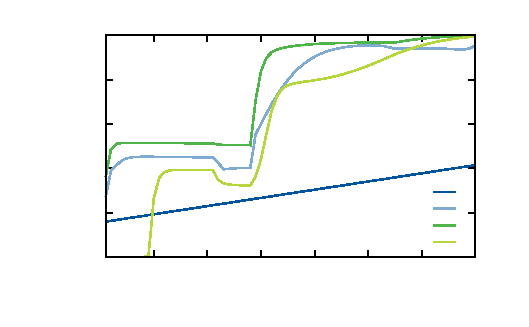
\includegraphics{GNUPlot/LPC_init_o2}}%
    \gplfronttext
  \end{picture}%
\endgroup

                \caption{oxygen concentration profiles.}
                \label{fig:lpc_example_o2}
            \end{subfigure}
            \hfill
            \begin{subfigure}{0.45\textwidth}
                % GNUPLOT: LaTeX picture with Postscript
\begingroup
  \makeatletter
  \providecommand\color[2][]{%
    \GenericError{(gnuplot) \space\space\space\@spaces}{%
      Package color not loaded in conjunction with
      terminal option `colourtext'%
    }{See the gnuplot documentation for explanation.%
    }{Either use 'blacktext' in gnuplot or load the package
      color.sty in LaTeX.}%
    \renewcommand\color[2][]{}%
  }%
  \providecommand\includegraphics[2][]{%
    \GenericError{(gnuplot) \space\space\space\@spaces}{%
      Package graphicx or graphics not loaded%
    }{See the gnuplot documentation for explanation.%
    }{The gnuplot epslatex terminal needs graphicx.sty or graphics.sty.}%
    \renewcommand\includegraphics[2][]{}%
  }%
  \providecommand\rotatebox[2]{#2}%
  \@ifundefined{ifGPcolor}{%
    \newif\ifGPcolor
    \GPcolortrue
  }{}%
  \@ifundefined{ifGPblacktext}{%
    \newif\ifGPblacktext
    \GPblacktexttrue
  }{}%
  % define a \g@addto@macro without @ in the name:
  \let\gplgaddtomacro\g@addto@macro
  % define empty templates for all commands taking text:
  \gdef\gplbacktext{}%
  \gdef\gplfronttext{}%
  \makeatother
  \ifGPblacktext
    % no textcolor at all
    \def\colorrgb#1{}%
    \def\colorgray#1{}%
  \else
    % gray or color?
    \ifGPcolor
      \def\colorrgb#1{\color[rgb]{#1}}%
      \def\colorgray#1{\color[gray]{#1}}%
      \expandafter\def\csname LTw\endcsname{\color{white}}%
      \expandafter\def\csname LTb\endcsname{\color{black}}%
      \expandafter\def\csname LTa\endcsname{\color{black}}%
      \expandafter\def\csname LT0\endcsname{\color[rgb]{1,0,0}}%
      \expandafter\def\csname LT1\endcsname{\color[rgb]{0,1,0}}%
      \expandafter\def\csname LT2\endcsname{\color[rgb]{0,0,1}}%
      \expandafter\def\csname LT3\endcsname{\color[rgb]{1,0,1}}%
      \expandafter\def\csname LT4\endcsname{\color[rgb]{0,1,1}}%
      \expandafter\def\csname LT5\endcsname{\color[rgb]{1,1,0}}%
      \expandafter\def\csname LT6\endcsname{\color[rgb]{0,0,0}}%
      \expandafter\def\csname LT7\endcsname{\color[rgb]{1,0.3,0}}%
      \expandafter\def\csname LT8\endcsname{\color[rgb]{0.5,0.5,0.5}}%
    \else
      % gray
      \def\colorrgb#1{\color{black}}%
      \def\colorgray#1{\color[gray]{#1}}%
      \expandafter\def\csname LTw\endcsname{\color{white}}%
      \expandafter\def\csname LTb\endcsname{\color{black}}%
      \expandafter\def\csname LTa\endcsname{\color{black}}%
      \expandafter\def\csname LT0\endcsname{\color{black}}%
      \expandafter\def\csname LT1\endcsname{\color{black}}%
      \expandafter\def\csname LT2\endcsname{\color{black}}%
      \expandafter\def\csname LT3\endcsname{\color{black}}%
      \expandafter\def\csname LT4\endcsname{\color{black}}%
      \expandafter\def\csname LT5\endcsname{\color{black}}%
      \expandafter\def\csname LT6\endcsname{\color{black}}%
      \expandafter\def\csname LT7\endcsname{\color{black}}%
      \expandafter\def\csname LT8\endcsname{\color{black}}%
    \fi
  \fi
  \setlength{\unitlength}{0.0500bp}%
  \begin{picture}(4762.00,2834.00)%
    \gplgaddtomacro\gplbacktext{%
      \csname LTb\endcsname%
      \put(758,512){\makebox(0,0)[r]{\strut{} 0.0}}%
      \put(758,938){\makebox(0,0)[r]{\strut{} 0.2}}%
      \put(758,1364){\makebox(0,0)[r]{\strut{} 0.4}}%
      \put(758,1789){\makebox(0,0)[r]{\strut{} 0.6}}%
      \put(758,2215){\makebox(0,0)[r]{\strut{} 0.8}}%
      \put(758,2641){\makebox(0,0)[r]{\strut{} 1.0}}%
      \put(1317,352){\makebox(0,0){\strut{} 10}}%
      \put(1831,352){\makebox(0,0){\strut{} 20}}%
      \put(2346,352){\makebox(0,0){\strut{} 30}}%
      \put(2860,352){\makebox(0,0){\strut{} 40}}%
      \put(3374,352){\makebox(0,0){\strut{} 50}}%
      \put(3889,352){\makebox(0,0){\strut{} 60}}%
      \put(4403,352){\makebox(0,0){\strut{} 70}}%
      \put(198,1576){\rotatebox{-270}{\makebox(0,0){\strut{}mole fraction $[-]$}}}%
      \put(2628,112){\makebox(0,0){\strut{}stage number $[\#]$}}%
    }%
    \gplgaddtomacro\gplfronttext{%
      \csname LTb\endcsname%
      \put(3908,1135){\makebox(0,0)[r]{\strut{}step 1}}%
      \csname LTb\endcsname%
      \put(3908,975){\makebox(0,0)[r]{\strut{}step 2}}%
      \csname LTb\endcsname%
      \put(3908,815){\makebox(0,0)[r]{\strut{}step 3}}%
      \csname LTb\endcsname%
      \put(3908,655){\makebox(0,0)[r]{\strut{}conv}}%
    }%
    \gplbacktext
    \put(0,0){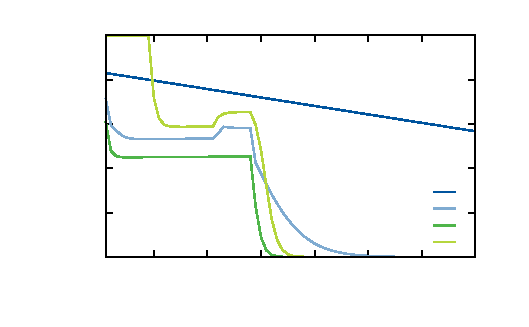
\includegraphics{GNUPlot/LPC_init_n2}}%
    \gplfronttext
  \end{picture}%
\endgroup

                \caption{nitrogen concentration profiles.}
                \label{fig:lpc_example_n2}
            \end{subfigure}
            \hspace{0.01\textwidth}
            \caption{initialization example concentration profiles.}
        \end{figure}

    \subsection{Steady-state optimization}
    Initially  optimizations were carried out using the steady-state process models.
    While an effort has been made to create a realistic scenario, the main focus of this section is to demonstrate
    optimization capabilities within the model environment \gproms and to compare different solution
    approaches for complex discrete-continuous problems.

        \subsubsection{Single steady-state operation}
        In a first case operations for two separate steady-states were optimized. However only structural
        decisions on the columns were made along with the columns operational parameters.
        %
        \begin{table}
            \center
            \footnotesize
            \rowcolors{2}{}{lightblue}
\begin{minipage}{\linewidth}
    \center
    \footnotesize
    \begin{tabular}{lrrrcrrr}
        & \multicolumn{3}{c}{steady state 1} & & \multicolumn{3}{c}{steady state 2} \\ \hline
        \rowcolor{white} variable name & result OA & result FB & deviation & & result OA & result FB & deviation \\ \hline
        \textbf{objective function} & \textbf{334702} & \textbf{328219} & \textbf{1.94 \%} & & \textbf{346320} & \textbf{346142} & \textbf{0.05 \%} \\
        plant air flowrate & 12434.6 & 11703.0 & 5.88 \% & & 12068.3 & 11981.1 & 0.72 \% \\
        CAC column diameter & 1.23543 & 1.16392 & 5.79 \% & & 1.10699 & 1.12137 & 1.30 \% \\
        CR CAC reflux ratio & 37.7408 & 33.6728 & 10.78 \% & & 39.6848 & 41.5425 & 4.68 \% \\
        CR main reflux ratio & 4.12825 & 3.80242 & 7.89 \% & & 2.54161 & 2.33128 & 8.28 \% \\
        HPC column diameter & 2.90256 & 2.80806 & 3.26 \% & & 2.88641 & 2.85296 & 1.16 \% \\
        HPC GN2 draw flowrate & 1945.52 & 1870.20 & 3.87 \% & & 532.432 & 839.935 & 57.75 \% \\
        LPC column diameter & 3.93352 & 3.79809 & 3.44 \% & & 4.13233 & 4.06009 & 1.75 \% \\
        waste draw flowrate & 7414.57 & 7082.99 & 4.47 \% & & 7088.12 & 7331.58 & 3.43 \% \\
        CAC draw flowrate & 738.246 & 662.048 & 10.32 \% & & 581.302 & 608.020 & 4.60 \% \\ \hline
    \end{tabular}
\end{minipage}

            \caption{steady-state optimization results - continuous variables.}
            \label{tab:ss_result_cont}
        \end{table}
        \begin{table}
            \center
            \footnotesize
            \rowcolors{2}{}{lightblue}
\begin{minipage}{\linewidth}
    \center
    \footnotesize
    \begin{tabular}{lcccccccc}
        & CAC N & HPC N & LPC N & LPC F1 & LPC F2 & LPC F3 & LPC S1 & LPC S2 \\ \hline
        steady-state 1 OA & 45 & 12 & 45 & 13 & 9 & 26 & 7 & 26 \\
        steady-state 1 FB & 44 & 13 & 47 & 10 & 7 & 23 & 6 & 23 \\
        steady-state 2 OA & 47 & 10 & 45 & 8 & 8 & 22 & 8 & 22 \\
        steady-state 2 FB & 45 & 12 & 46 & 8 & 6 & 21 & 6 & 21 \\ \hline
    \end{tabular}
\end{minipage}

            \caption{steady-state optimization results - discrete variables.}
            \label{tab:ss_result_disc}
        \end{table}
        \begin{table}
            \center
            \footnotesize
            \rowcolors{2}{}{lightblue}
\begin{minipage}{\linewidth}
    \center
    \footnotesize
    \begin{tabular}{lrrcrr}
        & \multicolumn{2}{c}{steady state 1} & & \multicolumn{2}{c}{steady state 2} \\ \hline
        \rowcolor{white} & results OA & results FB & & results OA & results FB \\ \hline
        total time [$s$] & 4847.88 & 1184.52 & & 2971.09 & 843.39 \\
        CPU time [$s$] & 26.72 & 225.72 & & 43.94 & 201.99 \\
        MINLP & 84 & 0 & & 68 & 0 \\
        NLP & 822 & 85 & & 687 & 68 \\
        line search steps & 2069 & 114 & & 1088 & 87 \\ \hline
    \end{tabular}
\end{minipage}


            \caption{steady-state optimization results - time consumption.}
            \label{tab:ss_result_time}
        \end{table}
        %
        The solutions from both algorithms are summarized in \tabref{tab:ss_result_cont} and \tabref{tab:ss_result_disc},
        where the for contains the results for all continuous decisions and the latter all discrete decisions. Results
        attained by outer approximation are labelled as ''OA'' and by solving the NCP as ''FB''.

        The objective function considers only capital cost for the separation sequence
        \Eq{eq:opt:ss_single_objective}{
            CAPEX = \left( \sum_c C_c^{\text{cap}} \right) \cdot \left(q^{-a} \frac{q^a - 1}{q - 1} \right),
                \eqannote{c = \left\{ \text{HPC}, \text{LPC}, \text{CAC}\right\} }.
        }
        %
        The difference between the steady-states lies in the requirements on product flow rates and purity. Hence the different
        constraints enforced for the respective operation modes are summarized in \tabref{tab:ss_constraints}.
        \begin{table}
            \center
            \footnotesize
            \rowcolors{2}{}{lightblue}
\begin{tabular}{lcrrcrr}
    & & \multicolumn{2}{c}{steady state 1} & & \multicolumn{2}{c}{steady state 2} \\
    \rowcolor{white} variable & & lower bound & upper bound & & lower bound & upper bound \\ \hline
    nitrogen product flowrate & & 3300 & 10000 & & 3000 & 10000 \\
    nitrogen product purity & & 0.999 & 1.0 & & 0.995 & 1.0 \\
    oxygen product flowrate & & 1700 & 10000 & & 1600 & 10000 \\
    oxygen product purity & & 0.995 & 1.0 & & 0.999 & 1.0 \\
    argon product flowrate & & 20 & 10000 & & 15 & 10000 \\
    argon product purity & & 0.995 & 1.0 & & 0.995 & 1.0 \\
    CAC diameter constraint & & 0 & 10 & & 0 & 10 \\
    LPC diameter constraint & & 0 & 10 & & 0 & 10 \\
    HPC diameter constraint & & 0 & 10 & & 0 & 10 
\end{tabular}

            \caption{steady-state optimization constraints.}
            \label{tab:ss_constraints}
        \end{table}

        When solving the continuous reformulation of the problem, an extra constraint for each integer variable in form of the
        relaxed Fischer-Burmeister function was added. Furthermore the closure condition for each location decision was added as
        an equality constraint. This closure condition needs not to be explicitly considered using the outer approximation approach,
        since this is handled internally by declaring so called special ordered sets of type one. This allows \gproms and the
        outer approximation algorithm to exploit the special structure of the problem due to the \emph{exclusive or} decisions.

        In order to compare the results of the different solution approaches, various aspects can be taken into consideration.
        Foremost the objective value is a measure of performance. As the complexity of the underlying problem increases,
        the matter of time becomes a -- sometimes limiting -- factor. Therefore the time in which a solution is found,
        is a measure for the algorithm performance as well. However before the results are discussed in greater detail,
        some further aspects are worth mentioning.

        In the process of solving the continuously reformulated problem, some difficulties arose. While
        (almost) integer values were found for most structural decisions, even during the initial iteration, especially
        the LPC column displayed some convergence problems. As the relaxation factor is reduced, the
        the feasible region between zero and one is is divided into two disjunct regions which become smaller and smaller.
        In some cases the solutions remain on one side of the feasible domain, namely the one converging to zero,
        while still fulfilling the closure constraint. As the relaxation factor is reduced, the solver is no longer able to
        ''make the jump'' to the other side of the domain. This leads to a distribution of small values for the split variables along
        the column. \Figref{fig:conv_fail} shows a typical example for this type of convergence behaviour. After the initial NLP the
        feed is somewhat evenly distributed between two stages, neither really dominant. As the relaxation is tightened, the values
        are reduced, and distributed among more stages to fulfil the closure condition. As the relaxation factor approaches zero the
        closure condition can no longer be satisfied, which leads to violation of the equality constraint and convergence failure.
        \begin{figure}
            \scriptsize
            \center
            % GNUPLOT: LaTeX picture with Postscript
\begingroup
  \makeatletter
  \providecommand\color[2][]{%
    \GenericError{(gnuplot) \space\space\space\@spaces}{%
      Package color not loaded in conjunction with
      terminal option `colourtext'%
    }{See the gnuplot documentation for explanation.%
    }{Either use 'blacktext' in gnuplot or load the package
      color.sty in LaTeX.}%
    \renewcommand\color[2][]{}%
  }%
  \providecommand\includegraphics[2][]{%
    \GenericError{(gnuplot) \space\space\space\@spaces}{%
      Package graphicx or graphics not loaded%
    }{See the gnuplot documentation for explanation.%
    }{The gnuplot epslatex terminal needs graphicx.sty or graphics.sty.}%
    \renewcommand\includegraphics[2][]{}%
  }%
  \providecommand\rotatebox[2]{#2}%
  \@ifundefined{ifGPcolor}{%
    \newif\ifGPcolor
    \GPcolortrue
  }{}%
  \@ifundefined{ifGPblacktext}{%
    \newif\ifGPblacktext
    \GPblacktexttrue
  }{}%
  % define a \g@addto@macro without @ in the name:
  \let\gplgaddtomacro\g@addto@macro
  % define empty templates for all commands taking text:
  \gdef\gplbacktext{}%
  \gdef\gplfronttext{}%
  \makeatother
  \ifGPblacktext
    % no textcolor at all
    \def\colorrgb#1{}%
    \def\colorgray#1{}%
  \else
    % gray or color?
    \ifGPcolor
      \def\colorrgb#1{\color[rgb]{#1}}%
      \def\colorgray#1{\color[gray]{#1}}%
      \expandafter\def\csname LTw\endcsname{\color{white}}%
      \expandafter\def\csname LTb\endcsname{\color{black}}%
      \expandafter\def\csname LTa\endcsname{\color{black}}%
      \expandafter\def\csname LT0\endcsname{\color[rgb]{1,0,0}}%
      \expandafter\def\csname LT1\endcsname{\color[rgb]{0,1,0}}%
      \expandafter\def\csname LT2\endcsname{\color[rgb]{0,0,1}}%
      \expandafter\def\csname LT3\endcsname{\color[rgb]{1,0,1}}%
      \expandafter\def\csname LT4\endcsname{\color[rgb]{0,1,1}}%
      \expandafter\def\csname LT5\endcsname{\color[rgb]{1,1,0}}%
      \expandafter\def\csname LT6\endcsname{\color[rgb]{0,0,0}}%
      \expandafter\def\csname LT7\endcsname{\color[rgb]{1,0.3,0}}%
      \expandafter\def\csname LT8\endcsname{\color[rgb]{0.5,0.5,0.5}}%
    \else
      % gray
      \def\colorrgb#1{\color{black}}%
      \def\colorgray#1{\color[gray]{#1}}%
      \expandafter\def\csname LTw\endcsname{\color{white}}%
      \expandafter\def\csname LTb\endcsname{\color{black}}%
      \expandafter\def\csname LTa\endcsname{\color{black}}%
      \expandafter\def\csname LT0\endcsname{\color{black}}%
      \expandafter\def\csname LT1\endcsname{\color{black}}%
      \expandafter\def\csname LT2\endcsname{\color{black}}%
      \expandafter\def\csname LT3\endcsname{\color{black}}%
      \expandafter\def\csname LT4\endcsname{\color{black}}%
      \expandafter\def\csname LT5\endcsname{\color{black}}%
      \expandafter\def\csname LT6\endcsname{\color{black}}%
      \expandafter\def\csname LT7\endcsname{\color{black}}%
      \expandafter\def\csname LT8\endcsname{\color{black}}%
    \fi
  \fi
  \setlength{\unitlength}{0.0500bp}%
  \begin{picture}(4762.00,1926.00)%
    \gplgaddtomacro\gplbacktext{%
      \csname LTb\endcsname%
      \put(686,320){\makebox(0,0)[r]{\strut{} 0.0}}%
      \put(686,603){\makebox(0,0)[r]{\strut{} 0.2}}%
      \put(686,885){\makebox(0,0)[r]{\strut{} 0.4}}%
      \put(686,1168){\makebox(0,0)[r]{\strut{} 0.6}}%
      \put(686,1450){\makebox(0,0)[r]{\strut{} 0.8}}%
      \put(686,1733){\makebox(0,0)[r]{\strut{} 1.0}}%
      \put(782,160){\makebox(0,0){\strut{} 1}}%
      \put(968,160){\makebox(0,0){\strut{} 2}}%
      \put(1154,160){\makebox(0,0){\strut{} 3}}%
      \put(1340,160){\makebox(0,0){\strut{} 4}}%
      \put(1526,160){\makebox(0,0){\strut{} 5}}%
      \put(1712,160){\makebox(0,0){\strut{} 6}}%
      \put(1898,160){\makebox(0,0){\strut{} 7}}%
      \put(2084,160){\makebox(0,0){\strut{} 8}}%
      \put(2270,160){\makebox(0,0){\strut{} 9}}%
      \put(2456,160){\makebox(0,0){\strut{} 10}}%
      \put(2641,160){\makebox(0,0){\strut{} 11}}%
      \put(2827,160){\makebox(0,0){\strut{} 12}}%
      \put(3013,160){\makebox(0,0){\strut{} 13}}%
      \put(3199,160){\makebox(0,0){\strut{} 14}}%
      \put(3385,160){\makebox(0,0){\strut{} 15}}%
      \put(3571,160){\makebox(0,0){\strut{} 16}}%
      \put(3757,160){\makebox(0,0){\strut{} 17}}%
      \put(3943,160){\makebox(0,0){\strut{} 18}}%
      \put(4129,160){\makebox(0,0){\strut{} 19}}%
      \put(4315,160){\makebox(0,0){\strut{} 20}}%
    }%
    \gplgaddtomacro\gplfronttext{%
    }%
    \gplbacktext
    \put(0,0){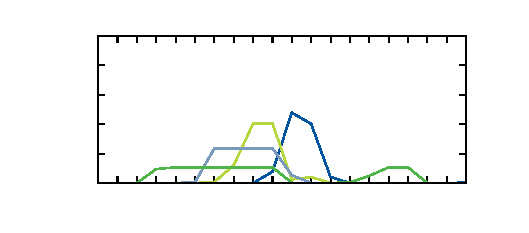
\includegraphics{GNUPlot/FB_converge}}%
    \gplfronttext
  \end{picture}%
\endgroup

            \caption{NCP convergence failure.}
            \label{fig:conv_fail}
        \end{figure}

        This issue has been addressed, by \cite{Kraemer.2010} who propose a re-initialization strategy based on the magnitude of
        the Lagrange multipliers associated with the continuous variables. While the results using this adjusted strategy
        are very promising it could not be implemented within the scope of this thesis. In addition to the adjusted algorithm,
        the problem formulation can be altered to improve convergence of the solution algorithm. Two strategies can
        be employed, which exploit the structure of the distillation model, or force the continuous solution to both sides
        of the feasible domain \cite{Kraemer.2009}.

        The first strategy involves reformulation of purity constraints in terms of the reflux split
        \Eq{}{
            \sum_j \zeta_j^R x_j \leq x_{\text{spec}}.
        }
        As one will always observe a concentration gradient in a finite distillation column, this formulation favours
        integer solutions as it competes with a lower capital costs which distributes fractions on lower trays. Hence
        this strategy is assumed to be most successful for steep concentration gradients at either of the column.
        It should be considered, that this formulation requires the variable tray location to be on the side at which
        the specified purity lies. \todo{write about optimization model.}

        The second approach relies on the previously introduced differentiable distribution function. Here a sufficient
        focus on a given tray can be enforced by adjusting the underlying standard deviation. By introducing that function
        in the first optimization stage, while continuing with the traditional formulation in the subsequent steps,
        convergence could be achieved.

        As for the optimization results. It can clearly be seen that both solution approaches return
        very similar objective values. However somewhat large deviations can be observed in the operational
        parameters and structural decisions. The deviations given in the results table are based on the results
        from the outer approximation. The fact that the optimal solutions deviate up to 57 \% in certain parameters
        further strengthes the argument, that due to the highly non-convex nature of the problem only locally optimal
        solutions are returned. Furthermore large differences can be seen in the computational time. While the
        total CPU time is considerably larger for the outer approximation algorithm, the CPU time is smaller.
        These results however depend heavily on the way the problem is posed. In the course of the thesis several
        different optimizations have been solved. Some with similar complexity as the cases discussed here.
        While the NCP always took comparable time for convergence, very large variations were observed,
        when the outer approximation algorithm was employed. For some cases solution times were even faster
        than the initial iteration of the NCP. Changes in this behaviour are most likely due to the
        quality of the linear approximations used to solve the MILP. Drastic changes could be observed
        when the feasible domain for certain decision variables was adjusted. Furthermore a considerable number
        of infeasible iterations was observed in the presented case. While in this case infeasible is
        not meant as violation of constraints but rather failure to converge the underlying process model after
        solving the MILP. To that regard several observations were made when working with the developed models.
        As initialization procedures are only carried out when simulating the process and not during optimizations,
        the solver has to initialize from an available previous solution or a saved variable set. For most cases,
        when the alteration in the process parameters are not too large, this posed no greater problem. Even changes in stream
        locations over several stages could be solved from available saved variable sets. However for
        some integer decisions convergence could fail by changing a stream location by only one tray.

        \subsubsection{Dual steady-state operation}
        For a second test case it was assumed, that the plant would have to operate under two distinct
        operation modes. One requiring a very high nitrogen purity and the other focusing on very pure oxygen.
        The steady states correspond to the ones from the previous section. To simultaneously consider two steady
        states, two instances of the process were were considered, that were allowed to differ in terms of operational decisions,
        but fixed in terms of structural decisions. The structural decisions are all stream locations and diameters.
        The decision variables correspond to the ones from the previous sections.

        This problem could only be converged using the reformulation strategy. The outer approximation algorithm
        did not converge for this particular case. However it needs to be pointed out, that a very similar case
        for somewhat less complex scenarios was converged by outer approximation. This particular case however could
        not even be solved using the optimal solution from the continuous reformulation as an initial guess.
        Nevertheless it is assumed, that with careful tweaking of the optimization parameters and solver setting
        convergence could eventually be achieved.
        Otherwise the same initial point as in the previous section was used to initialize the optimization.
        The results are summarized in \tabref{tab:ss_result_dual_cont} and \tabref{tab:ss_result_dual_disc}.
        \begin{table}
            \center
            \footnotesize
            \rowcolors{2}{}{lightblue}
\begin{minipage}{\linewidth}
    \center
    \footnotesize
    \begin{tabular}{lccccccccc}
        & amb. air & CR CAC $\nu$ & CR main $\nu$ & HPC SV 1 & LPC SV 1 & LPC SV 2 & CAC d & HPC d & LPC d \\ \hline
        mode 1 & 14135.58 & 28.869 & 4.2016 & 2064.272 & 8887.894 & 570.707 & 1.09 & 3.10 & 4.18\\
        mode 2 & 14974.81 & 89.664 & 4.4796 & 16.680 & 9999.85 & 1702.693 & - & - & - \\ \hline
    \end{tabular}
\end{minipage}

            \caption{dual steady-state optimization results - continuous variables.}
            \label{tab:ss_result_dual_cont}
        \end{table}
        \begin{table}
            \center
            \footnotesize
            \rowcolors{2}{}{lightblue}
\begin{minipage}{\linewidth}
    \center
    \footnotesize
    \begin{tabular}{lcccccccc}
        & CAC N & HPC N & LPC N & LPC F1 & LPC F2 & LPC F3 & LPC S1 & LPC S2 \\ \hline
        dual SS FB & 46 & 12 & 44 & 7 & 6 & 21 & 5 & 21 \\ \hline
    \end{tabular}
\end{minipage}

            \caption{dual steady-state optimization results - discrete variables.}
            \label{tab:ss_result_dual_disc}
        \end{table}

        As only one solution approach produced usable results, no comparison can be made as to the quality of the
        solution. However aside from from solution quality and time consumption, the robustness of a solution algorithm
        is very important, when it comes to solving complex scenarios. For the examples examined in the scope of this thesis,
        all problems which could be solved by outer approximation, could also be solved using the reformulation as NCP.
        In contrast, not all scenarios which where the NCP approach yielded a solution, could be solved by outer approximation.

        This suggests, that the reformulation strategy has are certain advantages in terms of robustness. It needs to be emphasised,
        that all findings here are limited to the narrow class of scenarios examined. Due to the limited range of problems, the findings
        deduced here have no claim for generality. Previous studies have shown \cite{Grossmann.2005} that the MINLP formulation
        of the separation sequence problem often yields (near) integer variables when solved as an NLP. This is due to the fact,
        that for each feed stream there is a distinct optimal stage. This stage corresponds to the one stage, where the concentration
        matches the feed concentration as closely as possible. By feeding a stream to such a stage, energy losses due to
        entropic mixing effects are minimized, and the need for external energy is kept to a minimum. This beneficial effect
        is not present for other integer decisions. The use of the DDF function or the reformulated purity constraint, as discussed
        in the previous section is also exclusive to distillation columns.


    \section{Dynamic models}
            The results of steady-state optimizations give very valuable information about the desired operation of
    the process in question. In real-live applications however, processes will always display transient behaviour,
    which cannot be captured by steady-state models. Even if the steady-state in question is in general a stable one,
    which means, that the process will return to the previous operation point given an external disturbance, process
    start-up and shut-down are in most cases still highly dynamic.

    The question of controlling a process is closely linked to the dynamic simulations. Any given process is required
    to operate within ceratin bounds and subject to external disturbances, which might cause the process to deviate
    from requirements on product specifications. To be able to handle such disturbances, or in some cases even be able
    to meet product requirements, control structures are implemented.

    The consideration of dynamics further opens the possibility to extend the optimization beyond monetary measures, or
    consider transient aspects which play a role in process profitability. This might include the optimization of transition
    times between multiple steady states, or an improved start-up or shut down behaviour. In case of the ASU which might also
    be implemented as a utility to a downstream process, the load following behaviour according to utility requirements could
    also be analyzed.

    In an effort to demonstrate dynamic optimization capabilities, several steps were taken. To be able to consider a control
    structure, controllers have to be implemented. Beyond that, as the control structure is not known a priori, a control
    superstructure has to be considered. The aim was to to optimize the control structure for a minimal transition time between
    the two steady-states considered during steady state optimization. The highly integrated nature of process leads to degrees
    freedom different from what would be expected from a regular distillation collum. Furthermore are they different
    from the steady-state case as described in \secref{sec:mathpro:steady:specinit}.

    \subsection{Degrees of freedom}
        In order to gain more insight into the behaviour of the dynamic models presented above an analysis
        of the degrees of freedom within the model is at hand. For the degrees of freedom the cost correlations
        will be disregarded, as they for a closed system of equations given the inputs generated form the column
        model. Furthermore interdependencies can be disregarded, as the cost model consist only of ''forward''
        computations. In practical terms this statement can be confirmed since the models can be evaluated
        with and without costing equations. Hence only the stage and hydraulic equations will be considered.

        For a given column without condenser or reboiler the model is made up of $[n_S (5n_C + 24) + n_F]$
        differential algebraic equations in $[n_S (5n_C + 29) + n_F (n_S + n_C + 3) + 1]$ variables. In this
        isolated case all feed flow rates, their composition and enthalpies would be specified. In this case
        the feeds include a hypothetical condenser reflux (the upper most feed) as well as reboiler reflux
        (lowest feed). Along with the feeds and their qualities, the feed splits and reflux split have to be
        assigned. Lastly the column diameter needs to be known. This yields $[n_F (n_S + n_C + 2) + n_S + 1]$
        specifications. To close the system initial conditions for all states have to be given. There
        are a total of $[4 n_S ]$ dynamic states in a column section.

        The condenser reboiler unit is made up of a total condenser and a reboiler side. For the condenser side
        holdups are neglected. While the reboiler side is modeled much like a column stage. The complete model
        consists of $[14 + 6 n_C]$ equations in $[17 + 6 n_C]$ variables. The three specified variables would
        commonly correspond to the condenser pressure, reboiler volume and reflux ratio on the condenser side.
        While other specifications are conceivable, they cannot be made entirely arbitrarily. A specification
        on the reboiler pressure for instance would result in a high index problem ($\approx n_S^{LPC}$) which
        could not be solved without drastically reformulating the model.

    \subsection{Dynamic process behaviour}
        With the dynamic models a more rigorous approach to analysing the process behaviour is possible.
        Several aspects of the transient behaviour are of interest. To gain an insight into the process dynamics
        and test the capabilities of the implemented models, several simulation studies have been conducted.

        Especially when dealing with control aspects of a process, the step responses to disturbances in the
        process are of great interest. Therefore first a study of process reactions to various internal and
        external disturbances will be conducted. This is followed by a more detailed investigation of some phenomena
        occurring during process operations.


        \subsubsection{Step responses}
            To identify a possible control structure the dynamic interactions of the process have to be analyzed.
            The most current method of controlling a process would be model predictive control (MPC), where
            the set point for all manipulated variables are provided by a central controller, which is based
            on a rigorous process model. In this case however a simpler and in practice still more common
            approach is to implement PID control loops. In that case each measured variable is paired
            with a manipulated variable, which is altered to keep the measured quantity within operational
            bounds.

            Among the most tested tools to synthesize a control structure are the relative gain array (RGA) and block
            relative gain (BRG). Those tools provide a measure for the interactions within the process. As it
            is unlikely, that one manipulated variable will only affect the controlled variable it is assigned to.
            Intuitively, highly integrated processes display strong interactions between all manipulated and
            measured variables. To properly calculate the RGA or BRG, a control (linearized) process model
            in terms of transfer functions is necessary. However, at this stage the requirement is not to find an
            optimal control structure, but rather a feasible one, which can be used as initial guess for
            optimization of the same.

            To derive feasible pairings, first all manipulated and measured variables are identified, based on the
            previously discussed degrees of freedom. The measured variables correspond to the constraints enforced
            on the process.
            \begin{itemize}
                \item LPC nitrogen purity $y_{1,N_2}^{LPC}$
                \item HPC nitrogen purity $y_{1,N_2}^{HPC}$
                \item oxygen product purity $x_{O_2}^{CR main}$
                \item CAC argon purity $y_{1,Ar}^{CAC}$
                \item nitrogen product flowrate $\dot{n}_{N_2}$
                \item oxygen product flowrate $\dot{n}_{O_2}$
                \item argon product flowrate $\dot{n}_{Ar}$
            \end{itemize}

            The manipulated variables are derived from the degrees of freedom analysis.
            \begin{itemize}
                \item main air feed flowrate $\dot{n}_{air}$
                \item CR main reflux ratio $\nu^{CR main}$
                \item CR CAC reflux ratio $\nu^{CR CAC}$
                \item HPC side stream flowrate $S^V_1$
                \item LPC side stream flowrate 1 $S^V_1$
                \item LPC side stream flowrate 2 $S^V_2$
            \end{itemize}

            To analyze the impact of the different manipulated variables, several simulation studies were
            undertaken. The steady state attained during steady state optimization was taken as nominal operating
            conditions. To get a feel for the process behaviour, the responses to a $10 \%$ step increase in
            the manipulated variables was simulated. The results are displayed in \figref{fig:opt:stepresp}.

            Before discussing the results in more detail, some comments have to be made as to how these results
            were attained, and how they are displayed. While for most cases the step response simulation was
            straightforward, it did lead to errors for the vapour side draw from the high pressure column. To still
            produce usable data, a steep ramp was used alternatively. Over a time-interval of 10 seconds, the nominal
            value was increased  by ten percent, and remained steady afterwards. To produce a meaningful and comparable
            representation of the simulation results, all values for the measured variables were normalized to their
            respective values under normal operating conditions. Furthermore there are two time scales employed, indicated
            on the bar below the graphs. All cases were simulated for the span of an entire day, and the step was applied
            at the very beginning of the simulation. When analysing the results, it turned out, that dynamic effects were
            taking place on two different scales. While some measured variables were only approaching steady-state
            at the end of the day, others reached it within about an hour. The different time scales are due to the
            nature of the measured variables. Pressure associated values such as flowrates change much more quickly,
            than temperature or concentrations \cite{Roffel.2000}. It also needs to be pointed out, that the y-scales
            for the graphs differ between measured variables. To maintain some degree or comparability,
            the y-scales are constant for each measured variable. In the given process configuration, the changes
            inflicted by the applied steps are of rather low amplitude. For the considered concentrations, the changes
            to the order of $10^-{3}$ or 0.1 \% were observed. Non the less, given these responses, preliminary candidates
            for coupling between controlled and measured variables can be obtained.

            \begin{landscape}
                \begin{figure}
                    \center
                    % GNUPLOT: LaTeX picture with Postscript
\begingroup
  \makeatletter
  \providecommand\rotatebox[2]{#2}%
  \@ifundefined{ifGPcolor}{%
    \newif\ifGPcolor
    \GPcolortrue
  }{}%
  \@ifundefined{ifGPblacktext}{%
    \newif\ifGPblacktext
    \GPblacktexttrue
  }{}%
  % define a \g@addto@macro without @ in the name:
  \let\gplgaddtomacro\g@addto@macro
  % define empty templates for all commands taking text:
  \gdef\gplbacktext{}%
  \gdef\gplfronttext{}%
  \makeatother
  
  \setlength{\unitlength}{1cm}%
  \begin{picture}(23.8,16)%
    \gplgaddtomacro\gplbacktext{%
        \put(0,1.75){\makebox(0,0)[r]{\strut{} $u_6$}}%
        \put(0,4.25){\makebox(0,0)[r]{\strut{} $u_5$}}%
        \put(0,6.75){\makebox(0,0)[r]{\strut{} $u_4$}}%
        \put(0,9.25){\makebox(0,0)[r]{\strut{} $u_3$}}%
        \put(0,11.75){\makebox(0,0)[r]{\strut{} $u_2$}}%
        \put(0,14.25){\makebox(0,0)[r]{\strut{} $u_1$}}%
        \put(2.4,16){\makebox(0,0)[cr]{\strut{} $y_1$}}%
        \put(6.2,16){\makebox(0,0)[cr]{\strut{} $y_2$}}%
        \put(10,16){\makebox(0,0)[cr]{\strut{} $y_3$}}%
        \put(13.8,16){\makebox(0,0)[cr]{\strut{} $y_4$}}%
        \put(17.6,16){\makebox(0,0)[cr]{\strut{} $y_5$}}%
        \put(21.4,16){\makebox(0,0)[cr]{\strut{} $y_6$}}%
        \put(0.5,0.25){\line(1,0){22.8}}
        \put(0.5,0.15){\line(0,1){0.2}}
        \put(4.3,0.15){\line(0,1){0.2}}
        \put(8.1,0.15){\line(0,1){0.2}}
        \put(11.9,0.15){\line(0,1){0.2}}
        \put(15.7,0.15){\line(0,1){0.2}}
        \put(19.5,0.15){\line(0,1){0.2}}
        \put(23.3,0.15){\line(0,1){0.2}}
        \put(2.4,0){\makebox(0,0)[c]{\strut{}  \footnotesize $1 d$}}%
        \put(6.2,0){\makebox(0,0)[c]{\strut{} \footnotesize $1 d$}}%
        \put(10,0){\makebox(0,0)[c]{\strut{} \footnotesize $1 d$}}%
        \put(13.8,0){\makebox(0,0)[c]{\strut{} \footnotesize $5000 s$}}%
        \put(17.6,0){\makebox(0,0)[c]{\strut{} \footnotesize $5000 s$}}%
        \put(21.4,0){\makebox(0,0)[c]{\strut{} \footnotesize $5000 s$}}%
    }%
    \gplgaddtomacro\gplfronttext{%
    }%
    \gplbacktext
    \put(0.5,0.5){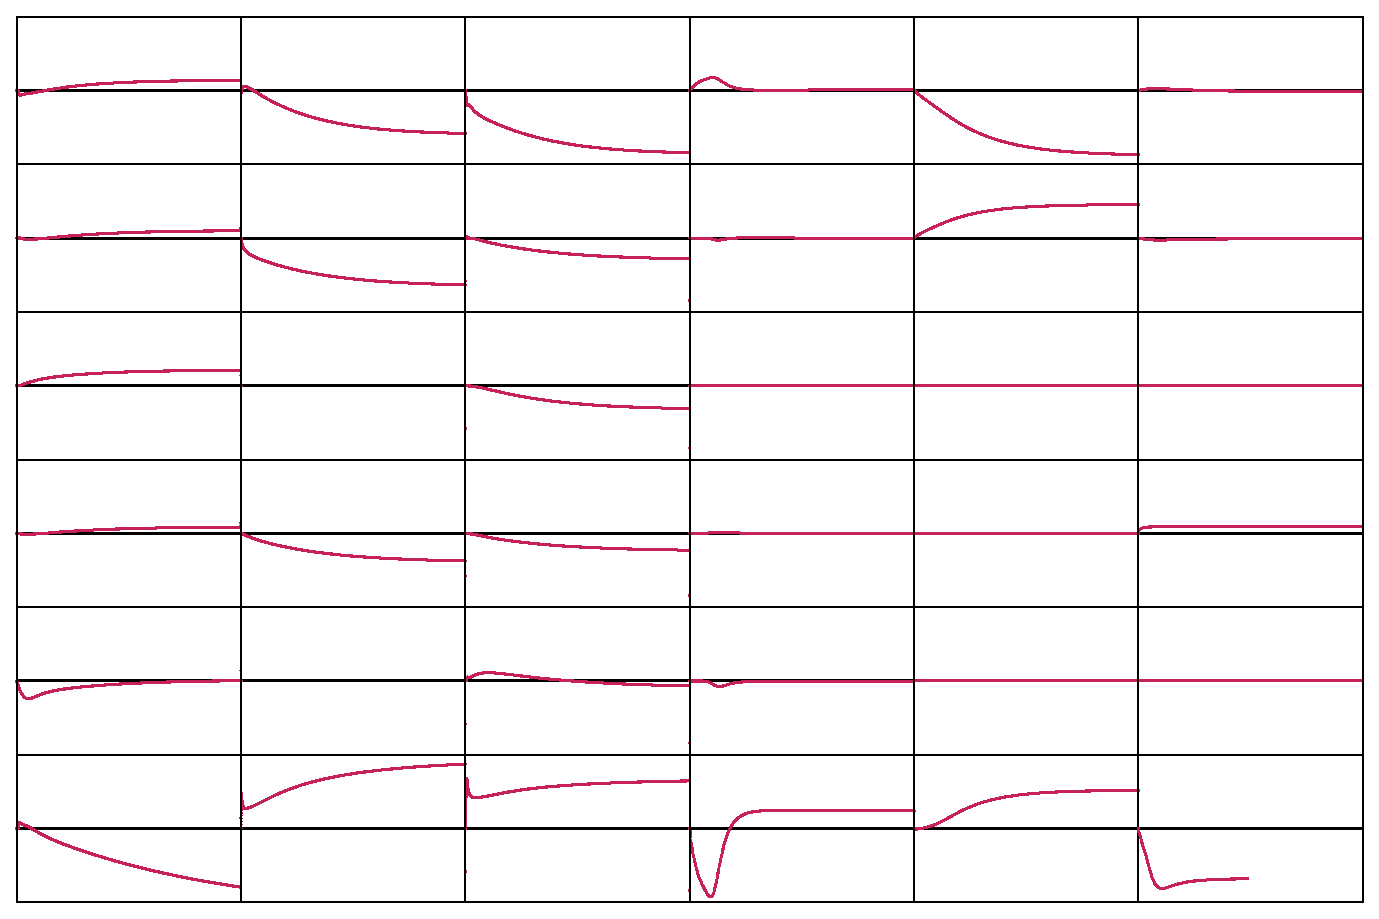
\includegraphics{GNUPlot/B1_Plot}}%
    \gplfronttext
  \end{picture}%
\endgroup

                    \caption{step responses.}
                    \label{fig:opt:stepresp}
                \end{figure}
            \end{landscape}



        \subsubsection{Dynamic profiles}
            The previous section showed only minor reactions to step changes in the manipulated variables. However
            a closer look at the dynamic column profiles reveals a much different picture. To analyze the internal
            column behaviour a external disturbance to the feed pressure was applied. As a result, the concentration
            profiles within the column undergo a various changes. Especially with high purity separation sequences,
            a highly non-linear behaviour with two distinct characteristics. For one, two time scales can
            be observed, in which new steady states are reached. Secondly, the transition time
            between two steady states relies heavily on the direction of the disturbance \cite{Hwang.1991}. The first
            effect deal with short- and long-term dynamics, while the second is referred to as asymmetric dynamics.

            \begin{figure}
                \scriptsize
                \center
                \begin{subfigure}{0.48\textwidth}
                    % GNUPLOT: LaTeX picture with Postscript
\begingroup
  \makeatletter
  \providecommand\color[2][]{%
    \GenericError{(gnuplot) \space\space\space\@spaces}{%
      Package color not loaded in conjunction with
      terminal option `colourtext'%
    }{See the gnuplot documentation for explanation.%
    }{Either use 'blacktext' in gnuplot or load the package
      color.sty in LaTeX.}%
    \renewcommand\color[2][]{}%
  }%
  \providecommand\includegraphics[2][]{%
    \GenericError{(gnuplot) \space\space\space\@spaces}{%
      Package graphicx or graphics not loaded%
    }{See the gnuplot documentation for explanation.%
    }{The gnuplot epslatex terminal needs graphicx.sty or graphics.sty.}%
    \renewcommand\includegraphics[2][]{}%
  }%
  \providecommand\rotatebox[2]{#2}%
  \@ifundefined{ifGPcolor}{%
    \newif\ifGPcolor
    \GPcolortrue
  }{}%
  \@ifundefined{ifGPblacktext}{%
    \newif\ifGPblacktext
    \GPblacktexttrue
  }{}%
  % define a \g@addto@macro without @ in the name:
  \let\gplgaddtomacro\g@addto@macro
  % define empty templates for all commands taking text:
  \gdef\gplbacktext{}%
  \gdef\gplfronttext{}%
  \makeatother
  \ifGPblacktext
    % no textcolor at all
    \def\colorrgb#1{}%
    \def\colorgray#1{}%
  \else
    % gray or color?
    \ifGPcolor
      \def\colorrgb#1{\color[rgb]{#1}}%
      \def\colorgray#1{\color[gray]{#1}}%
      \expandafter\def\csname LTw\endcsname{\color{white}}%
      \expandafter\def\csname LTb\endcsname{\color{black}}%
      \expandafter\def\csname LTa\endcsname{\color{black}}%
      \expandafter\def\csname LT0\endcsname{\color[rgb]{1,0,0}}%
      \expandafter\def\csname LT1\endcsname{\color[rgb]{0,1,0}}%
      \expandafter\def\csname LT2\endcsname{\color[rgb]{0,0,1}}%
      \expandafter\def\csname LT3\endcsname{\color[rgb]{1,0,1}}%
      \expandafter\def\csname LT4\endcsname{\color[rgb]{0,1,1}}%
      \expandafter\def\csname LT5\endcsname{\color[rgb]{1,1,0}}%
      \expandafter\def\csname LT6\endcsname{\color[rgb]{0,0,0}}%
      \expandafter\def\csname LT7\endcsname{\color[rgb]{1,0.3,0}}%
      \expandafter\def\csname LT8\endcsname{\color[rgb]{0.5,0.5,0.5}}%
    \else
      % gray
      \def\colorrgb#1{\color{black}}%
      \def\colorgray#1{\color[gray]{#1}}%
      \expandafter\def\csname LTw\endcsname{\color{white}}%
      \expandafter\def\csname LTb\endcsname{\color{black}}%
      \expandafter\def\csname LTa\endcsname{\color{black}}%
      \expandafter\def\csname LT0\endcsname{\color{black}}%
      \expandafter\def\csname LT1\endcsname{\color{black}}%
      \expandafter\def\csname LT2\endcsname{\color{black}}%
      \expandafter\def\csname LT3\endcsname{\color{black}}%
      \expandafter\def\csname LT4\endcsname{\color{black}}%
      \expandafter\def\csname LT5\endcsname{\color{black}}%
      \expandafter\def\csname LT6\endcsname{\color{black}}%
      \expandafter\def\csname LT7\endcsname{\color{black}}%
      \expandafter\def\csname LT8\endcsname{\color{black}}%
    \fi
  \fi
  \setlength{\unitlength}{0.0500bp}%
  \begin{picture}(4762.00,2834.00)%
    \gplgaddtomacro\gplbacktext{%
      \csname LTb\endcsname%
      \put(758,512){\makebox(0,0)[r]{\strut{} 0}}%
      \put(758,938){\makebox(0,0)[r]{\strut{} 0.2}}%
      \put(758,1364){\makebox(0,0)[r]{\strut{} 0.4}}%
      \put(758,1789){\makebox(0,0)[r]{\strut{} 0.6}}%
      \put(758,2215){\makebox(0,0)[r]{\strut{} 0.8}}%
      \put(758,2641){\makebox(0,0)[r]{\strut{} 1}}%
      \put(1177,352){\makebox(0,0){\strut{} 5}}%
      \put(1580,352){\makebox(0,0){\strut{} 10}}%
      \put(1983,352){\makebox(0,0){\strut{} 15}}%
      \put(2387,352){\makebox(0,0){\strut{} 20}}%
      \put(2790,352){\makebox(0,0){\strut{} 25}}%
      \put(3193,352){\makebox(0,0){\strut{} 30}}%
      \put(3596,352){\makebox(0,0){\strut{} 35}}%
      \put(4000,352){\makebox(0,0){\strut{} 40}}%
      \put(4403,352){\makebox(0,0){\strut{} 45}}%
      \put(198,1576){\rotatebox{-270}{\makebox(0,0){\strut{}mole fraction $[-]$}}}%
      \put(2628,112){\makebox(0,0){\strut{}stage number $[\#]$}}%
    }%
    \gplgaddtomacro\gplfronttext{%
      \csname LTb\endcsname%
      \put(3908,2498){\makebox(0,0)[r]{\strut{}$t = 0 s$}}%
      \csname LTb\endcsname%
      \put(3908,2338){\makebox(0,0)[r]{\strut{}$t = 2 \cdot 10^3 s$}}%
      \csname LTb\endcsname%
      \put(3908,2178){\makebox(0,0)[r]{\strut{}$t = 10^4 s$}}%
      \csname LTb\endcsname%
      \put(3908,2018){\makebox(0,0)[r]{\strut{}$t = 3 \cdot 10^4 s$}}%
    }%
    \gplbacktext
    \put(0,0){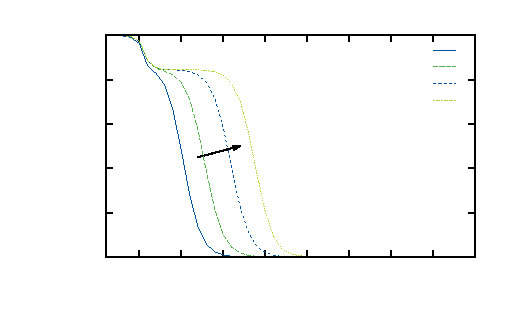
\includegraphics{GNUPlot/N2_ADyn_plus}}%
    \gplfronttext
  \end{picture}%
\endgroup

                    \caption{Dynamic profile after feed enthalpy increase.}
                    \label{fig:N2_ADyn_plus}
                \end{subfigure}
                    \begin{subfigure}{0.48\textwidth}
                    % GNUPLOT: LaTeX picture with Postscript
\begingroup
  \makeatletter
  \providecommand\color[2][]{%
    \GenericError{(gnuplot) \space\space\space\@spaces}{%
      Package color not loaded in conjunction with
      terminal option `colourtext'%
    }{See the gnuplot documentation for explanation.%
    }{Either use 'blacktext' in gnuplot or load the package
      color.sty in LaTeX.}%
    \renewcommand\color[2][]{}%
  }%
  \providecommand\includegraphics[2][]{%
    \GenericError{(gnuplot) \space\space\space\@spaces}{%
      Package graphicx or graphics not loaded%
    }{See the gnuplot documentation for explanation.%
    }{The gnuplot epslatex terminal needs graphicx.sty or graphics.sty.}%
    \renewcommand\includegraphics[2][]{}%
  }%
  \providecommand\rotatebox[2]{#2}%
  \@ifundefined{ifGPcolor}{%
    \newif\ifGPcolor
    \GPcolortrue
  }{}%
  \@ifundefined{ifGPblacktext}{%
    \newif\ifGPblacktext
    \GPblacktexttrue
  }{}%
  % define a \g@addto@macro without @ in the name:
  \let\gplgaddtomacro\g@addto@macro
  % define empty templates for all commands taking text:
  \gdef\gplbacktext{}%
  \gdef\gplfronttext{}%
  \makeatother
  \ifGPblacktext
    % no textcolor at all
    \def\colorrgb#1{}%
    \def\colorgray#1{}%
  \else
    % gray or color?
    \ifGPcolor
      \def\colorrgb#1{\color[rgb]{#1}}%
      \def\colorgray#1{\color[gray]{#1}}%
      \expandafter\def\csname LTw\endcsname{\color{white}}%
      \expandafter\def\csname LTb\endcsname{\color{black}}%
      \expandafter\def\csname LTa\endcsname{\color{black}}%
      \expandafter\def\csname LT0\endcsname{\color[rgb]{1,0,0}}%
      \expandafter\def\csname LT1\endcsname{\color[rgb]{0,1,0}}%
      \expandafter\def\csname LT2\endcsname{\color[rgb]{0,0,1}}%
      \expandafter\def\csname LT3\endcsname{\color[rgb]{1,0,1}}%
      \expandafter\def\csname LT4\endcsname{\color[rgb]{0,1,1}}%
      \expandafter\def\csname LT5\endcsname{\color[rgb]{1,1,0}}%
      \expandafter\def\csname LT6\endcsname{\color[rgb]{0,0,0}}%
      \expandafter\def\csname LT7\endcsname{\color[rgb]{1,0.3,0}}%
      \expandafter\def\csname LT8\endcsname{\color[rgb]{0.5,0.5,0.5}}%
    \else
      % gray
      \def\colorrgb#1{\color{black}}%
      \def\colorgray#1{\color[gray]{#1}}%
      \expandafter\def\csname LTw\endcsname{\color{white}}%
      \expandafter\def\csname LTb\endcsname{\color{black}}%
      \expandafter\def\csname LTa\endcsname{\color{black}}%
      \expandafter\def\csname LT0\endcsname{\color{black}}%
      \expandafter\def\csname LT1\endcsname{\color{black}}%
      \expandafter\def\csname LT2\endcsname{\color{black}}%
      \expandafter\def\csname LT3\endcsname{\color{black}}%
      \expandafter\def\csname LT4\endcsname{\color{black}}%
      \expandafter\def\csname LT5\endcsname{\color{black}}%
      \expandafter\def\csname LT6\endcsname{\color{black}}%
      \expandafter\def\csname LT7\endcsname{\color{black}}%
      \expandafter\def\csname LT8\endcsname{\color{black}}%
    \fi
  \fi
  \setlength{\unitlength}{0.0500bp}%
  \begin{picture}(4762.00,2834.00)%
    \gplgaddtomacro\gplbacktext{%
      \csname LTb\endcsname%
      \put(758,512){\makebox(0,0)[r]{\strut{} 0}}%
      \put(758,938){\makebox(0,0)[r]{\strut{} 0.2}}%
      \put(758,1364){\makebox(0,0)[r]{\strut{} 0.4}}%
      \put(758,1789){\makebox(0,0)[r]{\strut{} 0.6}}%
      \put(758,2215){\makebox(0,0)[r]{\strut{} 0.8}}%
      \put(758,2641){\makebox(0,0)[r]{\strut{} 1}}%
      \put(1177,352){\makebox(0,0){\strut{} 5}}%
      \put(1580,352){\makebox(0,0){\strut{} 10}}%
      \put(1983,352){\makebox(0,0){\strut{} 15}}%
      \put(2387,352){\makebox(0,0){\strut{} 20}}%
      \put(2790,352){\makebox(0,0){\strut{} 25}}%
      \put(3193,352){\makebox(0,0){\strut{} 30}}%
      \put(3596,352){\makebox(0,0){\strut{} 35}}%
      \put(4000,352){\makebox(0,0){\strut{} 40}}%
      \put(4403,352){\makebox(0,0){\strut{} 45}}%
      \put(198,1576){\rotatebox{-270}{\makebox(0,0){\strut{}mole fraction $[-]$}}}%
      \put(2628,112){\makebox(0,0){\strut{}stage number $[\#]$}}%
    }%
    \gplgaddtomacro\gplfronttext{%
      \csname LTb\endcsname%
      \put(3908,2498){\makebox(0,0)[r]{\strut{}$t = 0 s$}}%
      \csname LTb\endcsname%
      \put(3908,2338){\makebox(0,0)[r]{\strut{}$t = 2 \cdot 10^3 s$}}%
      \csname LTb\endcsname%
      \put(3908,2178){\makebox(0,0)[r]{\strut{}$t = 2 \cdot 10^3 s$}}%
      \csname LTb\endcsname%
      \put(3908,2018){\makebox(0,0)[r]{\strut{}$t = 10^4 s$}}%
    }%
    \gplbacktext
    \put(0,0){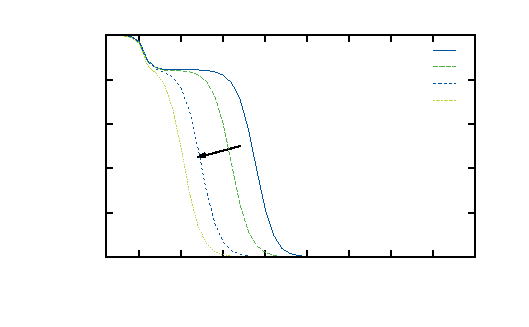
\includegraphics{GNUPlot/N2_ADyn_minus}}%
    \gplfronttext
  \end{picture}%
\endgroup

                    \caption{Dynamic profile after feed enthalpy decrease.}
                    \label{fig:N2_ADyn_minus}
                \end{subfigure}
            \end{figure}

            \begin{figure}
                \scriptsize
                \center
                \begin{subfigure}{0.48\textwidth}
                    % GNUPLOT: LaTeX picture with Postscript
\begingroup
  \makeatletter
  \providecommand\color[2][]{%
    \GenericError{(gnuplot) \space\space\space\@spaces}{%
      Package color not loaded in conjunction with
      terminal option `colourtext'%
    }{See the gnuplot documentation for explanation.%
    }{Either use 'blacktext' in gnuplot or load the package
      color.sty in LaTeX.}%
    \renewcommand\color[2][]{}%
  }%
  \providecommand\includegraphics[2][]{%
    \GenericError{(gnuplot) \space\space\space\@spaces}{%
      Package graphicx or graphics not loaded%
    }{See the gnuplot documentation for explanation.%
    }{The gnuplot epslatex terminal needs graphicx.sty or graphics.sty.}%
    \renewcommand\includegraphics[2][]{}%
  }%
  \providecommand\rotatebox[2]{#2}%
  \@ifundefined{ifGPcolor}{%
    \newif\ifGPcolor
    \GPcolortrue
  }{}%
  \@ifundefined{ifGPblacktext}{%
    \newif\ifGPblacktext
    \GPblacktexttrue
  }{}%
  % define a \g@addto@macro without @ in the name:
  \let\gplgaddtomacro\g@addto@macro
  % define empty templates for all commands taking text:
  \gdef\gplbacktext{}%
  \gdef\gplfronttext{}%
  \makeatother
  \ifGPblacktext
    % no textcolor at all
    \def\colorrgb#1{}%
    \def\colorgray#1{}%
  \else
    % gray or color?
    \ifGPcolor
      \def\colorrgb#1{\color[rgb]{#1}}%
      \def\colorgray#1{\color[gray]{#1}}%
      \expandafter\def\csname LTw\endcsname{\color{white}}%
      \expandafter\def\csname LTb\endcsname{\color{black}}%
      \expandafter\def\csname LTa\endcsname{\color{black}}%
      \expandafter\def\csname LT0\endcsname{\color[rgb]{1,0,0}}%
      \expandafter\def\csname LT1\endcsname{\color[rgb]{0,1,0}}%
      \expandafter\def\csname LT2\endcsname{\color[rgb]{0,0,1}}%
      \expandafter\def\csname LT3\endcsname{\color[rgb]{1,0,1}}%
      \expandafter\def\csname LT4\endcsname{\color[rgb]{0,1,1}}%
      \expandafter\def\csname LT5\endcsname{\color[rgb]{1,1,0}}%
      \expandafter\def\csname LT6\endcsname{\color[rgb]{0,0,0}}%
      \expandafter\def\csname LT7\endcsname{\color[rgb]{1,0.3,0}}%
      \expandafter\def\csname LT8\endcsname{\color[rgb]{0.5,0.5,0.5}}%
    \else
      % gray
      \def\colorrgb#1{\color{black}}%
      \def\colorgray#1{\color[gray]{#1}}%
      \expandafter\def\csname LTw\endcsname{\color{white}}%
      \expandafter\def\csname LTb\endcsname{\color{black}}%
      \expandafter\def\csname LTa\endcsname{\color{black}}%
      \expandafter\def\csname LT0\endcsname{\color{black}}%
      \expandafter\def\csname LT1\endcsname{\color{black}}%
      \expandafter\def\csname LT2\endcsname{\color{black}}%
      \expandafter\def\csname LT3\endcsname{\color{black}}%
      \expandafter\def\csname LT4\endcsname{\color{black}}%
      \expandafter\def\csname LT5\endcsname{\color{black}}%
      \expandafter\def\csname LT6\endcsname{\color{black}}%
      \expandafter\def\csname LT7\endcsname{\color{black}}%
      \expandafter\def\csname LT8\endcsname{\color{black}}%
    \fi
  \fi
  \setlength{\unitlength}{0.0500bp}%
  \begin{picture}(4762.00,2834.00)%
    \gplgaddtomacro\gplbacktext{%
      \csname LTb\endcsname%
      \put(758,512){\makebox(0,0)[r]{\strut{} 0.0}}%
      \put(758,938){\makebox(0,0)[r]{\strut{} 0.2}}%
      \put(758,1364){\makebox(0,0)[r]{\strut{} 0.4}}%
      \put(758,1789){\makebox(0,0)[r]{\strut{} 0.6}}%
      \put(758,2215){\makebox(0,0)[r]{\strut{} 0.8}}%
      \put(758,2641){\makebox(0,0)[r]{\strut{} 1.0}}%
      \put(1317,352){\makebox(0,0){\strut{} 10}}%
      \put(1831,352){\makebox(0,0){\strut{} 20}}%
      \put(2346,352){\makebox(0,0){\strut{} 30}}%
      \put(2860,352){\makebox(0,0){\strut{} 40}}%
      \put(3374,352){\makebox(0,0){\strut{} 50}}%
      \put(3889,352){\makebox(0,0){\strut{} 60}}%
      \put(4403,352){\makebox(0,0){\strut{} 70}}%
      \put(198,1576){\rotatebox{-270}{\makebox(0,0){\strut{}mole fraction $[-]$}}}%
      \put(2628,112){\makebox(0,0){\strut{}stage number $[\#]$}}%
    }%
    \gplgaddtomacro\gplfronttext{%
      \csname LTb\endcsname%
      \put(3908,655){\makebox(0,0)[r]{\strut{}step 1}}%
    }%
    \gplbacktext
    \put(0,0){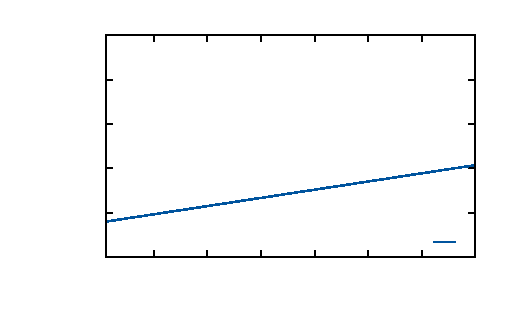
\includegraphics{GNUPlot/LPC_init_o2_s1}}%
    \gplfronttext
  \end{picture}%
\endgroup

                    \caption{Dynamic profile after feed enthalpy increase.}
                    \label{fig:N2_ADyn_plus}
                \end{subfigure}
                    \begin{subfigure}{0.48\textwidth}
                    % GNUPLOT: LaTeX picture with Postscript
\begingroup
  \makeatletter
  \providecommand\color[2][]{%
    \GenericError{(gnuplot) \space\space\space\@spaces}{%
      Package color not loaded in conjunction with
      terminal option `colourtext'%
    }{See the gnuplot documentation for explanation.%
    }{Either use 'blacktext' in gnuplot or load the package
      color.sty in LaTeX.}%
    \renewcommand\color[2][]{}%
  }%
  \providecommand\includegraphics[2][]{%
    \GenericError{(gnuplot) \space\space\space\@spaces}{%
      Package graphicx or graphics not loaded%
    }{See the gnuplot documentation for explanation.%
    }{The gnuplot epslatex terminal needs graphicx.sty or graphics.sty.}%
    \renewcommand\includegraphics[2][]{}%
  }%
  \providecommand\rotatebox[2]{#2}%
  \@ifundefined{ifGPcolor}{%
    \newif\ifGPcolor
    \GPcolortrue
  }{}%
  \@ifundefined{ifGPblacktext}{%
    \newif\ifGPblacktext
    \GPblacktexttrue
  }{}%
  % define a \g@addto@macro without @ in the name:
  \let\gplgaddtomacro\g@addto@macro
  % define empty templates for all commands taking text:
  \gdef\gplbacktext{}%
  \gdef\gplfronttext{}%
  \makeatother
  \ifGPblacktext
    % no textcolor at all
    \def\colorrgb#1{}%
    \def\colorgray#1{}%
  \else
    % gray or color?
    \ifGPcolor
      \def\colorrgb#1{\color[rgb]{#1}}%
      \def\colorgray#1{\color[gray]{#1}}%
      \expandafter\def\csname LTw\endcsname{\color{white}}%
      \expandafter\def\csname LTb\endcsname{\color{black}}%
      \expandafter\def\csname LTa\endcsname{\color{black}}%
      \expandafter\def\csname LT0\endcsname{\color[rgb]{1,0,0}}%
      \expandafter\def\csname LT1\endcsname{\color[rgb]{0,1,0}}%
      \expandafter\def\csname LT2\endcsname{\color[rgb]{0,0,1}}%
      \expandafter\def\csname LT3\endcsname{\color[rgb]{1,0,1}}%
      \expandafter\def\csname LT4\endcsname{\color[rgb]{0,1,1}}%
      \expandafter\def\csname LT5\endcsname{\color[rgb]{1,1,0}}%
      \expandafter\def\csname LT6\endcsname{\color[rgb]{0,0,0}}%
      \expandafter\def\csname LT7\endcsname{\color[rgb]{1,0.3,0}}%
      \expandafter\def\csname LT8\endcsname{\color[rgb]{0.5,0.5,0.5}}%
    \else
      % gray
      \def\colorrgb#1{\color{black}}%
      \def\colorgray#1{\color[gray]{#1}}%
      \expandafter\def\csname LTw\endcsname{\color{white}}%
      \expandafter\def\csname LTb\endcsname{\color{black}}%
      \expandafter\def\csname LTa\endcsname{\color{black}}%
      \expandafter\def\csname LT0\endcsname{\color{black}}%
      \expandafter\def\csname LT1\endcsname{\color{black}}%
      \expandafter\def\csname LT2\endcsname{\color{black}}%
      \expandafter\def\csname LT3\endcsname{\color{black}}%
      \expandafter\def\csname LT4\endcsname{\color{black}}%
      \expandafter\def\csname LT5\endcsname{\color{black}}%
      \expandafter\def\csname LT6\endcsname{\color{black}}%
      \expandafter\def\csname LT7\endcsname{\color{black}}%
      \expandafter\def\csname LT8\endcsname{\color{black}}%
    \fi
  \fi
  \setlength{\unitlength}{0.0500bp}%
  \begin{picture}(4762.00,2834.00)%
    \gplgaddtomacro\gplbacktext{%
      \csname LTb\endcsname%
      \put(758,512){\makebox(0,0)[r]{\strut{} 0.0}}%
      \put(758,938){\makebox(0,0)[r]{\strut{} 0.2}}%
      \put(758,1364){\makebox(0,0)[r]{\strut{} 0.4}}%
      \put(758,1789){\makebox(0,0)[r]{\strut{} 0.6}}%
      \put(758,2215){\makebox(0,0)[r]{\strut{} 0.8}}%
      \put(758,2641){\makebox(0,0)[r]{\strut{} 1.0}}%
      \put(1317,352){\makebox(0,0){\strut{} 10}}%
      \put(1831,352){\makebox(0,0){\strut{} 20}}%
      \put(2346,352){\makebox(0,0){\strut{} 30}}%
      \put(2860,352){\makebox(0,0){\strut{} 40}}%
      \put(3374,352){\makebox(0,0){\strut{} 50}}%
      \put(3889,352){\makebox(0,0){\strut{} 60}}%
      \put(4403,352){\makebox(0,0){\strut{} 70}}%
      \put(198,1576){\rotatebox{-270}{\makebox(0,0){\strut{}mole fraction $[-]$}}}%
      \put(2628,112){\makebox(0,0){\strut{}stage number $[\#]$}}%
    }%
    \gplgaddtomacro\gplfronttext{%
      \csname LTb\endcsname%
      \put(3908,815){\makebox(0,0)[r]{\strut{}step 1}}%
      \csname LTb\endcsname%
      \put(3908,655){\makebox(0,0)[r]{\strut{}step 2}}%
    }%
    \gplbacktext
    \put(0,0){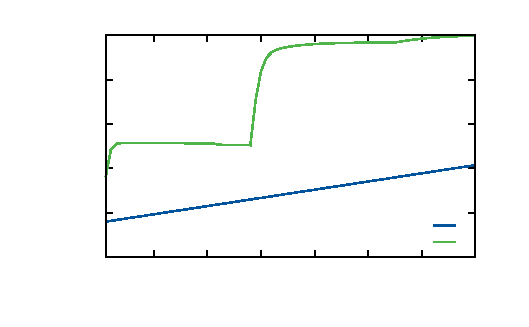
\includegraphics{GNUPlot/LPC_init_o2_s2}}%
    \gplfronttext
  \end{picture}%
\endgroup

                    \caption{Dynamic profile after feed enthalpy decrease.}
                    \label{fig:N2_ADyn_minus}
                \end{subfigure}
            \end{figure}

            \begin{figure}
                \scriptsize
                \center
                \begin{subfigure}{0.48\textwidth}
                    % GNUPLOT: LaTeX picture with Postscript
\begingroup
  \makeatletter
  \providecommand\color[2][]{%
    \GenericError{(gnuplot) \space\space\space\@spaces}{%
      Package color not loaded in conjunction with
      terminal option `colourtext'%
    }{See the gnuplot documentation for explanation.%
    }{Either use 'blacktext' in gnuplot or load the package
      color.sty in LaTeX.}%
    \renewcommand\color[2][]{}%
  }%
  \providecommand\includegraphics[2][]{%
    \GenericError{(gnuplot) \space\space\space\@spaces}{%
      Package graphicx or graphics not loaded%
    }{See the gnuplot documentation for explanation.%
    }{The gnuplot epslatex terminal needs graphicx.sty or graphics.sty.}%
    \renewcommand\includegraphics[2][]{}%
  }%
  \providecommand\rotatebox[2]{#2}%
  \@ifundefined{ifGPcolor}{%
    \newif\ifGPcolor
    \GPcolortrue
  }{}%
  \@ifundefined{ifGPblacktext}{%
    \newif\ifGPblacktext
    \GPblacktexttrue
  }{}%
  % define a \g@addto@macro without @ in the name:
  \let\gplgaddtomacro\g@addto@macro
  % define empty templates for all commands taking text:
  \gdef\gplbacktext{}%
  \gdef\gplfronttext{}%
  \makeatother
  \ifGPblacktext
    % no textcolor at all
    \def\colorrgb#1{}%
    \def\colorgray#1{}%
  \else
    % gray or color?
    \ifGPcolor
      \def\colorrgb#1{\color[rgb]{#1}}%
      \def\colorgray#1{\color[gray]{#1}}%
      \expandafter\def\csname LTw\endcsname{\color{white}}%
      \expandafter\def\csname LTb\endcsname{\color{black}}%
      \expandafter\def\csname LTa\endcsname{\color{black}}%
      \expandafter\def\csname LT0\endcsname{\color[rgb]{1,0,0}}%
      \expandafter\def\csname LT1\endcsname{\color[rgb]{0,1,0}}%
      \expandafter\def\csname LT2\endcsname{\color[rgb]{0,0,1}}%
      \expandafter\def\csname LT3\endcsname{\color[rgb]{1,0,1}}%
      \expandafter\def\csname LT4\endcsname{\color[rgb]{0,1,1}}%
      \expandafter\def\csname LT5\endcsname{\color[rgb]{1,1,0}}%
      \expandafter\def\csname LT6\endcsname{\color[rgb]{0,0,0}}%
      \expandafter\def\csname LT7\endcsname{\color[rgb]{1,0.3,0}}%
      \expandafter\def\csname LT8\endcsname{\color[rgb]{0.5,0.5,0.5}}%
    \else
      % gray
      \def\colorrgb#1{\color{black}}%
      \def\colorgray#1{\color[gray]{#1}}%
      \expandafter\def\csname LTw\endcsname{\color{white}}%
      \expandafter\def\csname LTb\endcsname{\color{black}}%
      \expandafter\def\csname LTa\endcsname{\color{black}}%
      \expandafter\def\csname LT0\endcsname{\color{black}}%
      \expandafter\def\csname LT1\endcsname{\color{black}}%
      \expandafter\def\csname LT2\endcsname{\color{black}}%
      \expandafter\def\csname LT3\endcsname{\color{black}}%
      \expandafter\def\csname LT4\endcsname{\color{black}}%
      \expandafter\def\csname LT5\endcsname{\color{black}}%
      \expandafter\def\csname LT6\endcsname{\color{black}}%
      \expandafter\def\csname LT7\endcsname{\color{black}}%
      \expandafter\def\csname LT8\endcsname{\color{black}}%
    \fi
  \fi
  \setlength{\unitlength}{0.0500bp}%
  \begin{picture}(4762.00,2834.00)%
    \gplgaddtomacro\gplbacktext{%
      \csname LTb\endcsname%
      \put(758,512){\makebox(0,0)[r]{\strut{} 0.0}}%
      \put(758,938){\makebox(0,0)[r]{\strut{} 0.2}}%
      \put(758,1364){\makebox(0,0)[r]{\strut{} 0.4}}%
      \put(758,1789){\makebox(0,0)[r]{\strut{} 0.6}}%
      \put(758,2215){\makebox(0,0)[r]{\strut{} 0.8}}%
      \put(758,2641){\makebox(0,0)[r]{\strut{} 1.0}}%
      \put(1317,352){\makebox(0,0){\strut{} 10}}%
      \put(1831,352){\makebox(0,0){\strut{} 20}}%
      \put(2346,352){\makebox(0,0){\strut{} 30}}%
      \put(2860,352){\makebox(0,0){\strut{} 40}}%
      \put(3374,352){\makebox(0,0){\strut{} 50}}%
      \put(3889,352){\makebox(0,0){\strut{} 60}}%
      \put(4403,352){\makebox(0,0){\strut{} 70}}%
      \put(198,1576){\rotatebox{-270}{\makebox(0,0){\strut{}mole fraction $[-]$}}}%
      \put(2628,112){\makebox(0,0){\strut{}stage number $[\#]$}}%
    }%
    \gplgaddtomacro\gplfronttext{%
      \csname LTb\endcsname%
      \put(3908,975){\makebox(0,0)[r]{\strut{}step 1}}%
      \csname LTb\endcsname%
      \put(3908,815){\makebox(0,0)[r]{\strut{}step 2}}%
      \csname LTb\endcsname%
      \put(3908,655){\makebox(0,0)[r]{\strut{}step 3}}%
    }%
    \gplbacktext
    \put(0,0){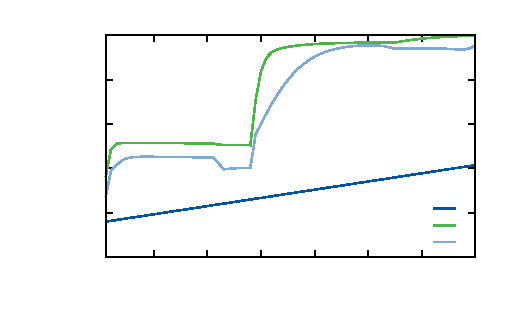
\includegraphics{GNUPlot/LPC_init_o2_s3}}%
    \gplfronttext
  \end{picture}%
\endgroup

                    \caption{Dynamic profile after feed enthalpy increase.}
                    \label{fig:N2_ADyn_plus}
                \end{subfigure}
                    \begin{subfigure}{0.48\textwidth}
                    % GNUPLOT: LaTeX picture with Postscript
\begingroup
  \makeatletter
  \providecommand\color[2][]{%
    \GenericError{(gnuplot) \space\space\space\@spaces}{%
      Package color not loaded in conjunction with
      terminal option `colourtext'%
    }{See the gnuplot documentation for explanation.%
    }{Either use 'blacktext' in gnuplot or load the package
      color.sty in LaTeX.}%
    \renewcommand\color[2][]{}%
  }%
  \providecommand\includegraphics[2][]{%
    \GenericError{(gnuplot) \space\space\space\@spaces}{%
      Package graphicx or graphics not loaded%
    }{See the gnuplot documentation for explanation.%
    }{The gnuplot epslatex terminal needs graphicx.sty or graphics.sty.}%
    \renewcommand\includegraphics[2][]{}%
  }%
  \providecommand\rotatebox[2]{#2}%
  \@ifundefined{ifGPcolor}{%
    \newif\ifGPcolor
    \GPcolortrue
  }{}%
  \@ifundefined{ifGPblacktext}{%
    \newif\ifGPblacktext
    \GPblacktexttrue
  }{}%
  % define a \g@addto@macro without @ in the name:
  \let\gplgaddtomacro\g@addto@macro
  % define empty templates for all commands taking text:
  \gdef\gplbacktext{}%
  \gdef\gplfronttext{}%
  \makeatother
  \ifGPblacktext
    % no textcolor at all
    \def\colorrgb#1{}%
    \def\colorgray#1{}%
  \else
    % gray or color?
    \ifGPcolor
      \def\colorrgb#1{\color[rgb]{#1}}%
      \def\colorgray#1{\color[gray]{#1}}%
      \expandafter\def\csname LTw\endcsname{\color{white}}%
      \expandafter\def\csname LTb\endcsname{\color{black}}%
      \expandafter\def\csname LTa\endcsname{\color{black}}%
      \expandafter\def\csname LT0\endcsname{\color[rgb]{1,0,0}}%
      \expandafter\def\csname LT1\endcsname{\color[rgb]{0,1,0}}%
      \expandafter\def\csname LT2\endcsname{\color[rgb]{0,0,1}}%
      \expandafter\def\csname LT3\endcsname{\color[rgb]{1,0,1}}%
      \expandafter\def\csname LT4\endcsname{\color[rgb]{0,1,1}}%
      \expandafter\def\csname LT5\endcsname{\color[rgb]{1,1,0}}%
      \expandafter\def\csname LT6\endcsname{\color[rgb]{0,0,0}}%
      \expandafter\def\csname LT7\endcsname{\color[rgb]{1,0.3,0}}%
      \expandafter\def\csname LT8\endcsname{\color[rgb]{0.5,0.5,0.5}}%
    \else
      % gray
      \def\colorrgb#1{\color{black}}%
      \def\colorgray#1{\color[gray]{#1}}%
      \expandafter\def\csname LTw\endcsname{\color{white}}%
      \expandafter\def\csname LTb\endcsname{\color{black}}%
      \expandafter\def\csname LTa\endcsname{\color{black}}%
      \expandafter\def\csname LT0\endcsname{\color{black}}%
      \expandafter\def\csname LT1\endcsname{\color{black}}%
      \expandafter\def\csname LT2\endcsname{\color{black}}%
      \expandafter\def\csname LT3\endcsname{\color{black}}%
      \expandafter\def\csname LT4\endcsname{\color{black}}%
      \expandafter\def\csname LT5\endcsname{\color{black}}%
      \expandafter\def\csname LT6\endcsname{\color{black}}%
      \expandafter\def\csname LT7\endcsname{\color{black}}%
      \expandafter\def\csname LT8\endcsname{\color{black}}%
    \fi
  \fi
  \setlength{\unitlength}{0.0500bp}%
  \begin{picture}(4762.00,2834.00)%
    \gplgaddtomacro\gplbacktext{%
      \csname LTb\endcsname%
      \put(758,512){\makebox(0,0)[r]{\strut{} 0.0}}%
      \put(758,938){\makebox(0,0)[r]{\strut{} 0.2}}%
      \put(758,1364){\makebox(0,0)[r]{\strut{} 0.4}}%
      \put(758,1789){\makebox(0,0)[r]{\strut{} 0.6}}%
      \put(758,2215){\makebox(0,0)[r]{\strut{} 0.8}}%
      \put(758,2641){\makebox(0,0)[r]{\strut{} 1.0}}%
      \put(1317,352){\makebox(0,0){\strut{} 10}}%
      \put(1831,352){\makebox(0,0){\strut{} 20}}%
      \put(2346,352){\makebox(0,0){\strut{} 30}}%
      \put(2860,352){\makebox(0,0){\strut{} 40}}%
      \put(3374,352){\makebox(0,0){\strut{} 50}}%
      \put(3889,352){\makebox(0,0){\strut{} 60}}%
      \put(4403,352){\makebox(0,0){\strut{} 70}}%
      \put(198,1576){\rotatebox{-270}{\makebox(0,0){\strut{}mole fraction $[-]$}}}%
      \put(2628,112){\makebox(0,0){\strut{}stage number $[\#]$}}%
    }%
    \gplgaddtomacro\gplfronttext{%
      \csname LTb\endcsname%
      \put(3908,1135){\makebox(0,0)[r]{\strut{}step 1}}%
      \csname LTb\endcsname%
      \put(3908,975){\makebox(0,0)[r]{\strut{}step 2}}%
      \csname LTb\endcsname%
      \put(3908,815){\makebox(0,0)[r]{\strut{}step 3}}%
      \csname LTb\endcsname%
      \put(3908,655){\makebox(0,0)[r]{\strut{}conv}}%
    }%
    \gplbacktext
    \put(0,0){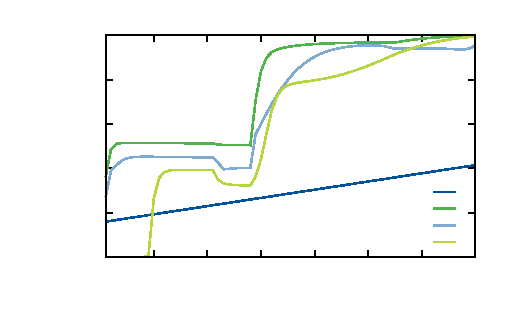
\includegraphics{GNUPlot/LPC_init_o2_s4}}%
    \gplfronttext
  \end{picture}%
\endgroup

                    \caption{Dynamic profile after feed enthalpy decrease.}
                    \label{fig:N2_ADyn_minus}
                \end{subfigure}
            \end{figure}







        
    \section{model application issues}
            Aside from the actual model equations care must be taken as to how to implement any set of equations,
    such that a numerical solver can find feasible solutions. The most prominent issues one is faced with in
    that context are scaling and singularities within the model. Both aspects will be briefly discussed here.

        \subsection{Scaling}
        When evaluating a model, or integrating over a given time span, Taylor expansion is used to construct
        an approximate linear process model. This means, that a system of the form
        \Eq{eq:lin_sys}{
            \vec{A} x = b,
        }
        is solved to a specified absolute accuracy $\varepsilon$. For a single equation the choice of an appropriate
        value for $\varepsilon$ is rather simple, given that the magnitude of $\vec{A} x$ and $b$ is known.
        Here one needs to consider, that if either magnitude is much grater than $\varepsilon$ a large number
        of iterations will be necessary to solve the system in question. On the other hand, if they are of similar
        magnitude relative error in the attained solution might become unacceptably high.

        To address these issues it is wise to consider the model scaling while implementing the equations.
        One approach would be to introduce scaling factors on both sides of an equation. While this
        may certainly improve scaling for the equation itself, the opposite might be true for the respective derivative.
        Consider the following simple example \cite{MarkPinto.2008} where to holdups are added to a total holdup
        \Eq{}{
            f(M_i) = M_1 + M_2 = M_T
        }
        Assuming both holdups are of magnitude $M_1 = M_2 = 10^5kg$, then the function value is $2 \cdot 10^5$, while for
        the derivative
        \Eq{}{
            \fracddpart{f}{M_1} = \fracddpart{f}{M_2} = \fracddpart{f}{M_T} = 1
        }
        holds. Introducing a scaling factor of $10^{-5}$ to both sides of the equation would lead to a function value
        of $2$ but have an adverse effect on the derivatives $\fracddpart{f}{M_i} = 10^{-5}$.

        A more robust approach would be to scale the units of the given equation which can simultaneously improve
        scaling for the function and its derivatives. Writing the same equation in tonnes would lead to  function value of
        $200$ while maintaining the well scaled derivatives. Alternatively one can introduce further variables and equations
        with the aim to get more linear equation and rescale some parts of the original equation. A more linear function
        leads to more constant Jacobian elements and reduces the need for Jacobian updates which can be very expensive in
        computational terms.
        
        When it comes to the dynamic models, the issue of scaling is extend with another aspect. While for the steady-state
        models, one could rewrite each equation with different units, as long as each equation is in itself consistent, 
        the same cannot be said, for the dynamic models. Here it is imperative, to maintain the same time scale for every 
        dynamic equation. Due to the very large flow-rates, the steady-state and dynamic balances were written in 
        $\frac{kmol}{hr}$ to achieve a well scaled equation. Considering the various dynamic effects discussed in 
        the previous section, this seems to coarse to capture all relevant phenomena. Maintaining one time unit as one 
        hour would lead to integrator steps of $\frac{1}{3600}$ for one second. Considering furthermore the small changes 
        in the model variables, intuitively this would lead to very badly scaled problems. To somehow accommodate these 
        considerations, it was decided, to introduce a scaling factor solely on the left hand side of the dynamic equations. 
        By those means, the time scale of the process model can easily be adjusted for seconds, minutes, hours or days.  

        \subsection{Singularities}
        Singularities in the models considered here often occur, when a variable is raised to a non-integer power,
        or the logarithm of a variable is evaluated.
        Expressions like have no solution within the rational domain, when the respective variable becomes negative.
        Furthermore when negative exponents are involved a value of zero would lead to a division by zero which is
        undefined. Even before that the function value might become very large as the variable approaches zero.

        In the context of a distillation column, this issue becomes especially relevant, when optimizations or simulations
        with inactive trays are carried out. Some flowrates in the inactive section of the model will be zero, depending
        on whether the top or bottom reflux is optimized, those will be either vapour or liquid flowrates. While a
        solution of zero might cause issues in some cases, a negative solution introduces even more complications. As the
        equations are solved within numerical accuracy, this might also lead to (slightly) negative solutions, which will
        cause the numerical solver to fail. Such scenarios have to be anticipated while implementing the model and
        appropriate measures have to be taken to ''protect'' such variables from hindering model evaluation.

        As \gproms supports state transition networks, one way is to introduce conditional statements. However
        those statements will in almost all cases lead to discontinuities in the model. While in principal such
        discontinuities can be detected by numerical solvers \cite{Pantelides.2003}, they are a further source
        for instabilities. Hence they should in the best case only be introduces, when there is a physical correspondence
        in the system behaviour.

        In this thesis the problem was approached by decoupling the flowrates within the column, and the ones used for evaluation
        of the hydraulic model. With the help of the split fractions active and inactive trays can be distinguished.
        \Eq{}{
            V_j^{\text{hyd}} = \left( \sum_{k=1}^j \zeta^R_k \right) \cdot V_j + \left(1 - \left( \sum_{k=1}^j \zeta^R_k \right)\right) \cdot V_1
        }
        Here it should be pointed out, that it only needs to be ensured, the the hydraulic model can be evaluated for inactive trays.
        What results are returned for these trays has no effect for the modelled column operation.
